%%%%%%%%%%% INFORMAÇÕES BÁSICAS %%%%%%%%%%%%%%%
% Versão: 1.2
% Autores:  Rafael Lima
%	        Rodrigo Guimarães
% Finalidade: Curso de Escrita em LaTeX
%%%%%%%%%%% FIM INFORMAÇÕES BÁSICAS %%%%%%%%%%%


% !TEX encoding = UTF-8 Unicode
% !TEX TS-program = pdflatex

%%%%%%%%%%% INCLUSÃO DE PACOTES %%%%%%%%%%%%%%%%
% Tipo: Apresentação de Slides
% Opcional: svgnames - Garantir cores
\documentclass[svgnames]{beamer}
% Formatação no padrão EdSoc
\usepackage{Layout/beamerEdSoc}
\usepackage{amsmath, amssymb, array}



%%%%%%%%%%% INFORMAÇÕES INICIAIS %%%%%%%%%%%%%%
\title[O Preparador de~Documentos \LaTeX]{\LARGE{\textbf{Preparador~de~Documentos \LaTeX}}}
  \subtitle{Introdução}
\author{Rafael Lima \and \\
        Rodrigo Guimarães}
\institute{UnB/EdSoc}
\date {\today}
%%%%%%%%%%% FIM INFORMAÇÕES INICIAIS %%%%%%%%%%

%%%%%%%%%%% DOCUMENTO %%%%%%%%%%%%%%%%%%%%%%%%%
\begin{document}

%%%%%%%%%%% PRÓLOGO %%%%%%%%%%%%%%%%%%%%%%%%%%%
% NÃO EXCLUIR
%%%%%%%%%%% INTRODUÇÃO %%%%%%%%%%%%%%%%%%%%%%

%%%%%%%%%%% FINALIDADE %%%%%%%%%%%%%%%%%%%%%%
%	Unir todas as informações básicas e 
%	inerentes ao conteúdo do resto da
%	apresentação, principalmente ao se tratar
%	de uma apresentação para um curso
%%%%%%%%%%% FIM FINALIDADE %%%%%%%%%%%%%%%%%%

%	Informções básicas do arquivo, título
\begin{frame}[plain]
  \maketitle
\end{frame}

%	Licença
\begin{frame}{Licença GNU FDL}
	Copyright \copyright\ 2005--2013 Carlos A. P. Campani.\nn
 	É garantida a permissão para copiar, distribuir e/ou modificar este documento sob os termos da Licença de Documentação Livre GNU (GNU Free Documentation License), Versão 1.2 ou qualquer versão posterior publicada pela Free Software Foundation; sem Seções Invariantes, Textos de Capa Frontal, e sem Textos de Quarta Capa. Uma cópia da licença é incluída na seção intitulada ``GNU Free Documentation License''.\nn
	veja:~\scriptsize{\url{http://www.ic.unicamp.br/~norton/fdl.html}}.
\end{frame}

%	Nota Especial
\begin{frame}{Nota}
	Apresentação adaptada do Curso de Latex disponível no pacote Texlive. Agradeço aos professores Campani e Beccari da Universidade Federal de Campinas, pela qualidade do conteúdo original pelo suporte no prepáro do curso e orientação quanto ao uso dos slides.\nn
	veja:~\scriptsize{\url{http://www.tug.org/texlive/devsrc/Master/texmf-dist/doc/latex/cursolatex/cursolatex.pdf}}.
\end{frame}

%	Bibliografia
\begin{frame}{Bibliografia}
  \begin{thebibliography}{1}
    \bibitem {bib:lamport} Lamport, Leslie \emph{\LaTeX: A Document Preparation System}, Addison-Wesley Publishing Company, 2nd edition, 1994.
    \bibitem {bib:goossens} Goossens, Michel and Mittelbach, Frank and Samarin, Alexander \emph{The \LaTeX Companion}, Addison-Wesley, 2.a ed, 2004.
    \bibitem {bib:campani}\ Campani and Beccari \emph{Introdução ao~Uso do~Preparador~de~Documentos \LaTeX}, 2011
  \end{thebibliography}
\end{frame}

%	Links Importantes
\begin{frame}{Links}
  \begin{itemize}
    \item Comunidade de Usuários \scriptsize{\url{http://www.tug.org/}}
    \item \normalsize{\TeX\ Live Homepage: }\scriptsize{\url{http://www.tug.org/texlive/}}
    \item \normalsize{MiK\TeX{} Project: }\scriptsize{\url{http://www.miktex.org}}
    \item \normalsize{CTAN -- The Comprehensive \TeX\ Archive Network: }\scriptsize{\url{http://www.ctan.org/}}
    \item \normalsize{\LaTeX{} Project Page: }\scriptsize{\url{http://www.latex-project.org/}}
    \item \normalsize{Wikibook (en): }\scriptsize{\url{http://en.wikibooks.org/wiki/LaTeX}}
  \end{itemize}
\end{frame}

%	Documentos e Tutorias Importantes
\begin{frame}{Documentos e tutoriais}
	\begin{itemize}
		\item \emph{Introdução ao \LaTeXe}, Tobias Oetiker, Hubert Partl, Irene Hyna and Elisabeth Schlegl\n\scriptsize{\url{http://www.ufpel.tche.br/~campani/lshortBR.pdf}}
		\item \normalsize{\TeX\ Tutoriais: }\scriptsize{\url{http://www.tug.org/tutorials/tugindia/}}
		\item \normalsize{Lâminas do curso}%\scriptsize{\url{https://github.com/Mecajun/Curso_LaTeX/blob/master/cursolatex.pdf?raw=true}}
	\end{itemize}
\end{frame}
%%%%%%%%%%% FIM INTRODUÇÃO %%%%%%%%%%%%%%%%%%

%%%%%%%%%%% INSTALAÇÃO %%%%%%%%%%%%%%%%%%%%%%%%
%\section{Instalação}
%\input{Conteudos/InstalacaoLatex.tex}

%%%%%%%%%%% FORMATAÇÃO GERAL P0 %%%%%%%%%%%%%%%
%\section{Aula 1}
%%%%%%%%%%%%%%%%%%%%%%%%%% AULA 01 %%%%%%%%%%%%%%%%%%%%%%%%%%

%%%%%%%%%%%%%%%%%%%%%%% FINALIDADE %%%%%%%%%%%%%%%%%%%%%%%%%%
%			Tratar das explicações básicas sobre o			%
%			TeX e LaTeX, apontando as principais			%
%			vantagens sobre os métodos comuns para a 		%
%			diagramação de documentos, além de demonstrar	%
%			comandos sobre formatação geral de documentos	%
%%%%%%%%%%%%%%%%%%%%%%% FIM FINALIDADE %%%%%%%%%%%%%%%%%%%%%%

%%%%%%%%%%% SLIDE 01 %%%%%%%%%%%%%%%%%%%%%%%%
\begin{frame}{O que é o \TeX?}
	\begin{itemize}
		\item \TeX~é um programa criado por Donald E.~Knuth, usado para desenvolvimento de documentos;
		\pause
		\item Formatador de documentos (como troff e groff -- programas hoje obsoletos);
	\end{itemize}
\end{frame}
%%%%%%%%%%% FIM SLIDE 01 %%%%%%%%%%%%%%%%%%%%

%%%%%%%%%%% SLIDE 02 %%%%%%%%%%%%%%%%%%%%%%%%
\begin{frame}{O que faz o \TeX?}
	\begin{itemize}
		\item Permite desenvolver documentos complexos, incluindo facilidades para:
		\pause
	\begin{itemize}
		\item Gerar sumário, index, lista de figuras, lista de tabelas e referências bibliográficas;
		\pause		
		\item Importar e tratar imagens de vários formatos  (escalando, rotacionando, convertendo, etc.);
		\pause
		\item Desenvolver gráficos diagramáticos;
		\pause
		\item Representar partituras musicais, partidas de xadrez, fórmulas químicas, dentre outros.
	\end{itemize}
\end{itemize}

	\pause
	\begin{Observacao}{O poder do \TeX}
		Reside em sua habilidade de tratar textos técnicos complicados e exibir fórmulas matemáticas.
	\end{Observacao}
\end{frame}
%%%%%%%%%%% FIM SLIDE 02 %%%%%%%%%%%%%%%%%%%%

%%%%%%%%%%% SLIDE 03 %%%%%%%%%%%%%%%%%%%%%%%%
\begin{frame}{Vantagens}
	\begin{itemize}
		\item Qualidade tipográfica superior (fontes e distribuição do texto na página);
		\pause
		\item Compatibilidade (Donald Knuth ``congelou'' o programa \TeX);
		\pause
		\item Estabilidade e ausência de falhas (uso prolongado do mesmo programa virtualmente eliminou todos os erros);
		\pause
		\item Padrão adotado pela \emph{American Mathematical Society} (AMS) para comunicação entre matemáticos;
		\pause
		\item Quantidade extremamente vasta de pacotes mantidos pela comunidade para facilitar qualquer tarefa.
	\end{itemize}
\end{frame}
%%%%%%%%%%% FIM SLIDE 03 %%%%%%%%%%%%%%%%%%%%%

%%%%%%%%%%% SLIDE 04 %%%%%%%%%%%%%%%%%%%%%%%%%
\begin{frame}{O que é \LaTeX?}
	\begin{itemize}
		\item \LaTeX\ é um conjunto padrão de macros para \TeX\ que permite um aumento da produtividade no uso do programa;
		\pause
		\item Mais macros podem ser incluidas por meio de pacotes (por exemplo: \Xy-pic, MusiX\TeX, CircuiTikz, etc.);
		\pause
		\item Programas externos, desenvolvidos por programadores e usuários de \TeX, extenderam as funcionalidades (por exemplo: BiB\TeX, makeindex, etc.).
	\end{itemize}
\end{frame}
%%%%%%%%%%% FIM SLIDE 04 %%%%%%%%%%%%%%%%%%%%%

%%%%%%%%%%% SLIDE 05 %%%%%%%%%%%%%%%%%%%%%%%%%
\begin{frame}{Abordagens para o projeto de documentos}
	\begin{itemize}
		\item Projeto visual $\times$ projeto lógico de documentos:
		\pause
		\begin{itemize}
			\item Projeto visual enfatiza o estético e envolve grande esforço de formatação;
			\pause
			\item Projeto lógico enfatiza a estrutura e economiza tempo pois a formatação é consequência da estrutura;
			\pause
			\item Projeto lógico provoca uma reflexão sobre o texto que tem consequências benéficas até sobre o conteúdo sendo desenvolvido;
		\end{itemize}
	\end{itemize}
\end{frame}
%%%%%%%%%%% FIM SLIDE 05 %%%%%%%%%%%%%%%%%%%%%

%%%%%%%%%%% SLIDE 06 %%%%%%%%%%%%%%%%%%%%%%%%%
\begin{frame}{Comparação entre processador de textos e \TeX}
	Fórmula obtida usando-se um processador de textos típico:
	\pause
	\begin{center}
		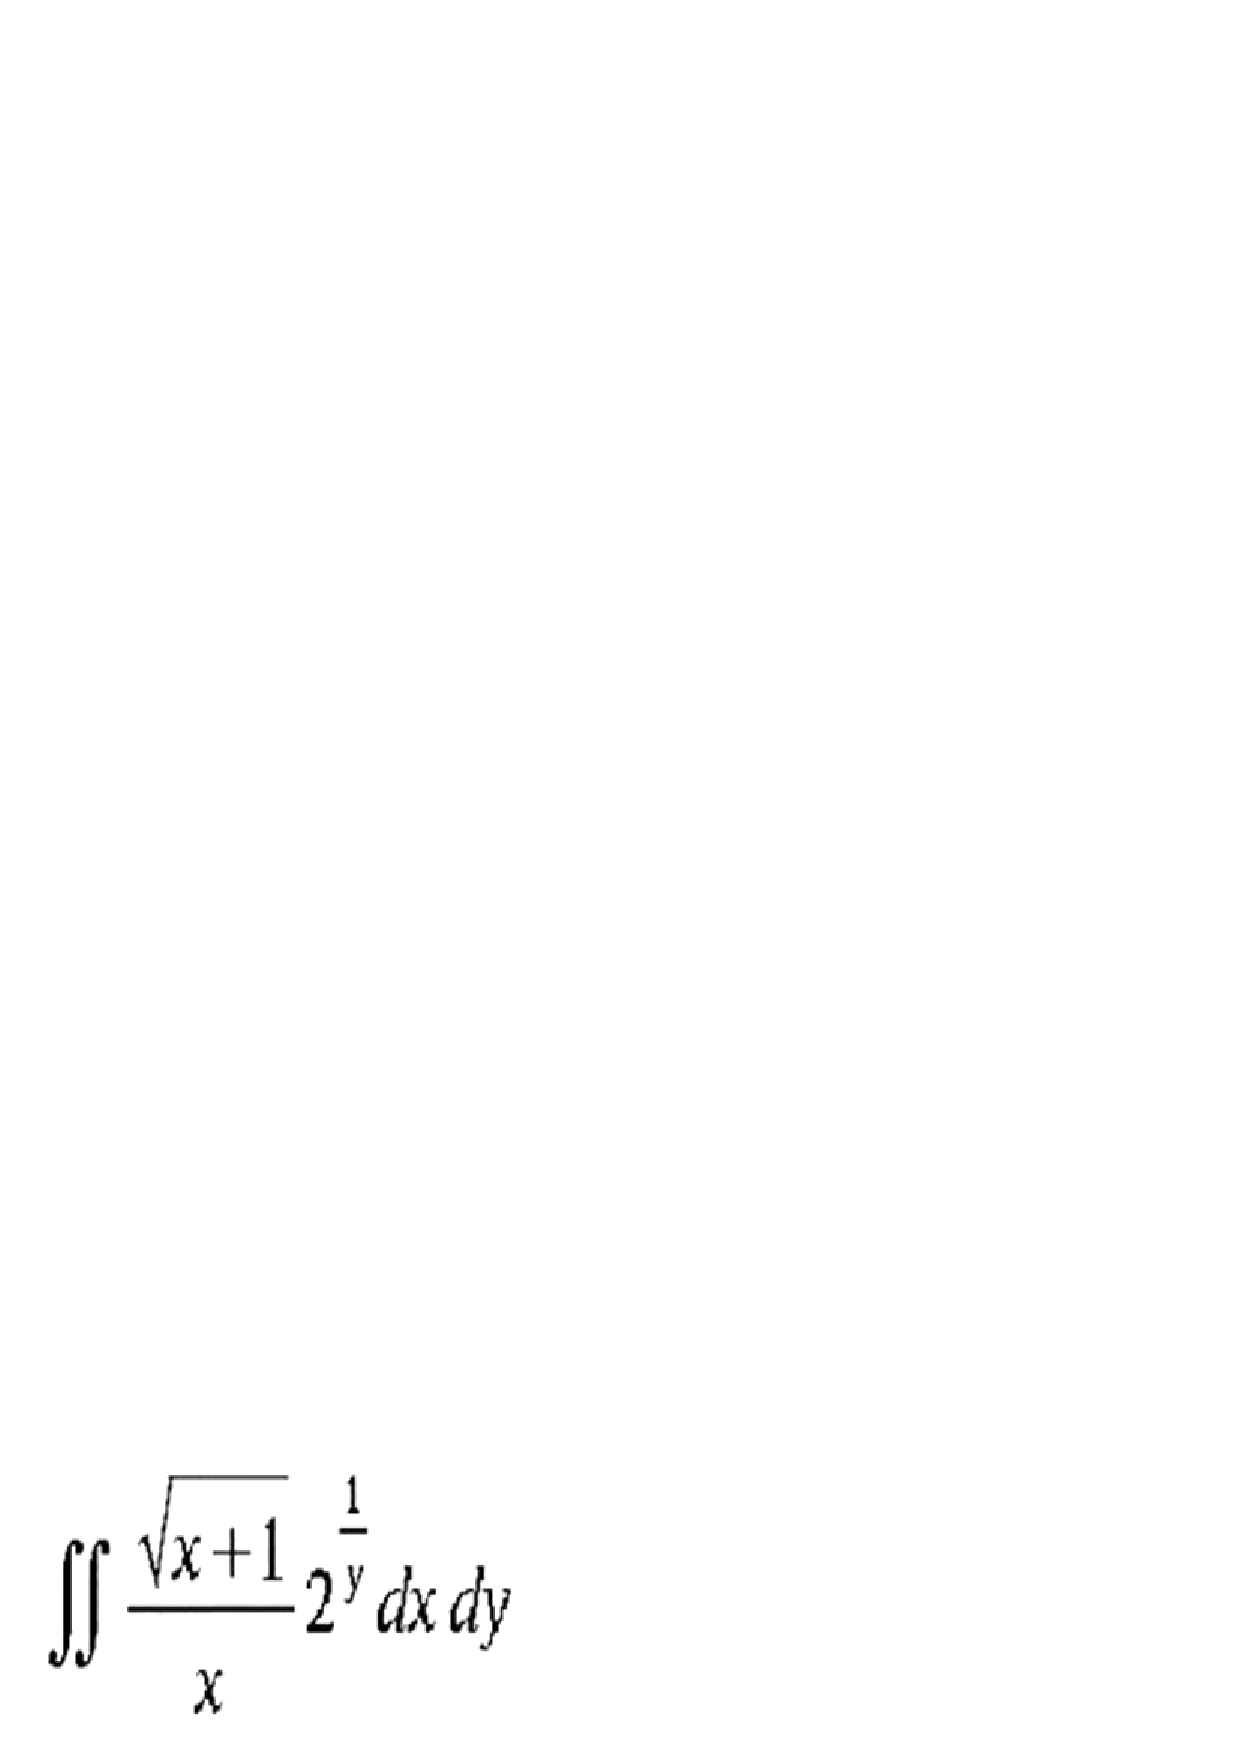
\includegraphics[width=0.5\textwidth, natwidth=326, natheight=175]{Imagens/integral.png}
	\end{center}

    \pause
	Fórmula obtida usando-se \TeX:
	\pause
	\[\int\!\!\!\int\frac{\sqrt{x+1}}{x}2^{\frac{1}{y}}\mathrm{d}x\,\mathrm{d}y\]
\end{frame}
%%%%%%%%%%% FIM SLIDE 06 %%%%%%%%%%%%%%%%%%%%%

%%%%%%%%%%% SLIDE 07 %%%%%%%%%%%%%%%%%%%%%%%%%
\begin{frame}{Projeto visual $\times$ lógico}
	\begin{description}
		\item [Projeto visual] baseado em menus e botões (o usuário ``desenha'' a fórmula/texto);
		\pause
		\item [Projeto lógico] baseado em comandos:
	\end{description}
	
	\pause
	
	\begin{Codigo}{Comandos}
		\string\[\LCmd{int}\string\!\string\!\string\!\LCmd{int}
		\LCmdArg{frac}{\LCmdArg{sqrt}{x+1}}\Larg{x}2\string^\{
		\LCmdArg{frac}{1}\Larg{y}\}\n
		\LCmdArg{mathrm}{d}x\string\,\LCmdArg{mathrm}{d}y\string\]
	\end{Codigo}

    \pause
	Produz:
    \begin{Resultado}{}
		\[\int\!\!\!\int\frac{\sqrt{x+1}}{x}2^{\frac{1}{y}}\mathrm{d}x\,\mathrm{d}y\]
    \end{Resultado}
\end{frame}
%%%%%%%%%%% FIM SLIDE 07 %%%%%%%%%%%%%%%%%%%%%

%%%%%%%%%%% SLIDE 08 %%%%%%%%%%%%%%%%%%%%%%%%%
\begin{frame}{Observações}
	\begin{itemize}
		\item \texttt{\string\[ } e \texttt{\string\]} -- entra e sai do modo matemático;
		\item \LCmd{int} -- integral;
		\item \texttt{\string\!} -- espaço negativo (para obter o espaçamento correto na integral dupla) -- poderia ter sido usado o comando \LCmd{iint};
		\item \LCmdArg{frac}{\ldots}\Larg{\ldots} -- fração;
		\item \LCmdArg{sqrt}{\ldots} -- raiz quadrada;
		\item \texttt{\string^} -- expoente;
		\item \texttt{\string\,} -- espaço pequeno;
		\item \LCmdArg{mathrm}{\ldots} -- fonte romano do modo matemático.
	\end{itemize}
\end{frame}
%%%%%%%%%%% FIM SLIDE 08 %%%%%%%%%%%%%%%%%%%%%

%%%%%%%%%%% SLIDE 09 %%%%%%%%%%%%%%%%%%%%%%%%%
\begin{frame}{Projeto lógico}
	\begin{itemize}
		\item No projeto lógico, o aspecto estético depende do contexto/estrutura (por exemplo, se a fórmula está dentro de um parágrafo ou destacada do parágrafo). 
		Exemplo:
		\begin{itemize}
			\item O somatório $\sum_{i = 0}^\infty a_i/2$ resulta em \dots
			\pause	
			\item O somatório $$\sum_{i = 0}^\infty \frac{a_i}{2}$$ resulta em \dots
		\end{itemize}
	\end{itemize}
\end{frame}
%%%%%%%%%%% FIM SLIDE 09 %%%%%%%%%%%%%%%%%%%%%

%%%%%%%%%%% FORMATAÇÃO GERAL P1 %%%%%%%%%%%%%%%
%\section{Aula 1}
%%%%%%%%%%%%%%%%%%%%%%%%%% AULA 01 %%%%%%%%%%%%%%%%%%%%%%%%%%

%%%%%%%%%%%%%%%%%%%%%%% FINALIDADE %%%%%%%%%%%%%%%%%%%%%%%%%%
%			Tratar da estrutura dos comandos em LaTeX   	%
%			e TeX, apontando os principais recursos para	%
%			diagramação de documentos, além de demonstrar	%
%			comandos sobre formatação geral de documentos	%
%%%%%%%%%%%%%%%%%%%%%%% FIM FINALIDADE %%%%%%%%%%%%%%%%%%%%%%

%%%%%%%%%%% SLIDE 10 %%%%%%%%%%%%%%%%%%%%%%%%%
\begin{frame}{Os comandos do \LaTeX}
	\begin{itemize}
		\item Os comandos são necessários para que \LaTeX\ possa formatar o texto (\LaTeX\ não é tão inteligente como um designer/tipógrafo humano);
		\pause
		\item Os comandos \TeX\ normalmente são antecedidos de ``\texttt{\textbackslash}'' (por exemplo, para obter \LaTeX\ deve-se digitar \LCmd{LaTeX} e para obter ``\textbackslash'' deve-se digitar \texttt{\$}\LCmd{backslash}\texttt{\$} ou \LCmd{textbackslash});
		\pause
		\item A linguagem \TeX\ segue as regras/ideias de linguagens de programação (declarações e corpo do programa; ligação de bibliotecas; regras de escopo; etc.);
	\end{itemize}
	
    \begin{Observacao}{Observação}
	    Maiúsculas $\neq$ minúsculas.
    \end{Observacao}
\end{frame}
%%%%%%%%%%% FIM SLIDE 10 %%%%%%%%%%%%%%%%%%%%%

%%%%%%%%%%% SLIDE 11 %%%%%%%%%%%%%%%%%%%%%%%%%
\begin{frame}[fragile=singleslide]{Compilando, visualizando e imprimindo}
	Comandos para o Terminal do Linux:
	\begin{itemize}
		\item Compilação: \verb'$ pdflatex teste.tex' (para compilar, por exemplo, o arquivo \verb'teste.tex');
		\pause
		\item *Visualização: \verb'$ xdg-open teste.pdf' (o arquivo é recarregado automaticamente a cada modificação). Em alguns programas o resultado em .PDF aparece direitamente numa segunda janela;
		\pause
		\item Convertendo para html: \verb'$ latex2html teste.tex' (necessita instalar o comando);
		\pause
		\item Imprimindo: \verb'$ dvips teste.dvi' ou \verb'$ lpr teste.ps'.
	\end{itemize}
\end{frame}
%%%%%%%%%%% FIM SLIDE 11 %%%%%%%%%%%%%%%%%%%%%

%%%%%%%%%%% SLIDE 12 %%%%%%%%%%%%%%%%%%%%%%%%%
\begin{frame}{Estrutura e comandos \LaTeX}
	\begin{Codigo}{Estrutura geral}
		\LCmdOptArg{documentclass}{opcionais}{classe}\n
			~declarações~\dots\n
		\LCmdArg{begin}{document}\n
			~documento~\dots\n
		\LCmdArg{end}{document}
	\end{Codigo}

\medskip

	\begin{Codigo}{Para trabalhar com arquivos grandes}
		\LCmdArg{include}{nomearquivo}
			\% inclui comandos de um arquivo\n \% gera nova página antes\nn
		\LCmdArg{input}{nomearquivo} 
			\% inclui comandos de um arquivo\n \% não gera nova página
	\end{Codigo}
\end{frame}
%%%%%%%%%%% FIM SLIDE 12 %%%%%%%%%%%%%%%%%%%%%

%%%%%%%%%%% SLIDE 13 %%%%%%%%%%%%%%%%%%%%%%%%%
\begin{frame}{Estrutura dos comandos}
	\begin{itemize}
		\item Comandos \LaTeX{} são normalmente precedidos por \texttt{\textbackslash} e seguidos de parâmetros opcionais (delimitados por ``\texttt{[}`` e ``\texttt{]}'') e/ou parâmetros obrigatórios (delimitados por ``\texttt{\lb}'' e ``\texttt{\rb}'');
		\pause
		\begin{Codigo}{Exemplos}
			\LCmd{TeX}\n
			\LCmd{LaTeX}\n
			\LCmdArg{documentclass}{book}\n
			\LCmdOptArg{documentclass}{12pt}{article}\n
			\LCmdArg{begin}{document}
		\end{Codigo}
\bigskip
		\pause
		\item Uma excessão a esta regra é ``\texttt{\$}'' que delimita o ambiente matemático. Exemplo: \texttt{\$3+2\LCmdArg{sqrt}{2}\$}, que produz $3+2\sqrt{2}$.
	\end{itemize}
\end{frame}
%%%%%%%%%%% FIM SLIDE 13 %%%%%%%%%%%%%%%%%%%%%

%%%%%%%%%%% SLIDE 14 %%%%%%%%%%%%%%%%%%%%%%%%%
\begin{frame}{Espaços após um comando \TeX}
	Espaços após um comando serão consumidos até encontrar um caracter diferente de branco, resultando que
	\pause
		\begin{Codigo}{}
			\LCmd{TeX} é legal!
		\end{Codigo}
		
	\pause
	Produz:
	
		\begin{Resultado}{}
			\TeX é legal!
		\end{Resultado}
	\pause
	Para evitar isto, use \texttt{\textbackslash\textvisiblespace}\footnote{O símbolo \texttt{\textvisiblespace}  serve para representar o espaço no texto fonte.} ou \texttt{\{\}}, que interrompe o consumo de espaços em branco, ou \texttt{\textasciitilde} (espaço em branco indivisível):

	\pause
	\begin{Codigo}{}
		\LCmd{TeX}\textbackslash\textvisiblespace é legal!\n
		ou\n
		\LCmd{TeX}\{\}\textvisiblespace é legal!\n
		ou\n
		\LCmd{TeX}\textasciitilde é legal!
	\end{Codigo}
\end{frame}
%%%%%%%%%%% FIM SLIDE 14 %%%%%%%%%%%%%%%%%%%%%

%%%%%%%%%%% SLIDE 15 %%%%%%%%%%%%%%%%%%%%%%%%%
\begin{frame}{Sobre espaçamento}\fontsize{10}{12}\selectfont
	\begin{itemize}
		\item Para produzir espaço no texto pode-se usar ``\LCmd{\textvisiblespace}'', que representa o espaço simples;
		\pause
		\item Para produzir espaço negativo: \texttt{\string\!};
		\pause
		\item ``\texttt{\textasciitilde}'' produz um espaço que não pode ser dividido em uma quebra de linha; por exemplo: \texttt{fone:\ (61)\textasciitilde5551234};
		\pause
		\item \TeX\ assume que sentenças terminam com ``.'', introduzindo um espaço adicional ao final da frase. O comando \LCmd{frenchspacing} desabilita este espaço adicional;
		\pause
		\item Para obter espaço vertical: \LCmdArg{vspace}{espaço} (não permite obter espaço no início de uma página) e \LCmdArg{vspace*}{espaço} (conserva o espaço no início de uma página);
		\pause
		\item \LCmdArg{hspace}{espaço} permite obter espaço horizontal dentro de uma linha;
		\pause
		\item Pode-se usar as dimensões em pontos (pt), polegadas (in), milímetros (mm), centímetros (cm) etc.
	\end{itemize}
\end{frame}
%%%%%%%%%%% FIM SLIDE 15 %%%%%%%%%%%%%%%%%%%%%

%%%%%%%%%%% SLIDE EXTRA %%%%%%%%%%%%%%%%%%%%%%
\begin{frame}{Conversão de medidas}
    \tiny
    \begin{center}\begin{tabular} % Tabela da NASA, gerada automaticamente pelo LaTeX
      {>{\def\colunit{pt}}l<{\convertto{\rowunit}{1\colunit}}
       >{\def\colunit{mm}}l<{\convertto{\rowunit}{1\colunit}}
       >{\def\colunit{cm}}l<{\convertto{\rowunit}{1\colunit}}
       >{\def\colunit{ex}}l<{\convertto{\rowunit}{1\colunit}}
       >{\def\colunit{bp}}l<{\convertto{\rowunit}{1\colunit}}
       >{\def\colunit{pc}}l<{\convertto{\rowunit}{1\colunit}}
       >{\def\colunit{in}}l<{\convertto{\rowunit}{1\colunit}}
       >{\bfseries}l}
       \hline
    \multicolumn{1}{l}{\bfseries 1pt} & \multicolumn{1}{l}{\bfseries 1mm} & \multicolumn{1}{l}{\bfseries 1cm} & \multicolumn{1}{l}{\bfseries 1ex} & \multicolumn{1}{l}{\bfseries 1bp} & \multicolumn{1}{l}{\bfseries 1pc} & \multicolumn{1}{l}{\bfseries 1in} & \\
    \gdef\rowunit{pt} & & & & & & & \rowunit\\
    \gdef\rowunit{mm} & & & & & & & \rowunit\\
    \gdef\rowunit{cm} & & & & & & & \rowunit\\
    \gdef\rowunit{ex} & & & & & & & \rowunit\\
    \gdef\rowunit{bp} & & & & & & & \rowunit\\
    \gdef\rowunit{pc} & & & & & & & \rowunit\\
    \gdef\rowunit{in} & & & & & & & \rowunit\\
    \hline
    \end{tabular}\end{center}
\end{frame}
%%%%%%%%%%% FIM SLIDE EXTRA %%%%%%%%%%%%%%%%%%

%%%%%%%%%%% SLIDE 16 %%%%%%%%%%%%%%%%%%%%%%%%%
\begin{frame}{Delimitação de parágrafos}
	Uma ou mais linhas em branco delimita os parágrafos:
	\pause
	\begin{Codigo}{Exemplo}
		Este é o\textvisiblespace\textvisiblespace\textvisiblespace\textvisiblespace primeiro \n parágrafo.\n

		E este é o segundo!
	\end{Codigo}

	\pause
	Produz:
	\begin{Resultado}{}
		Este é o         primeiro
		parágrafo.

		E este é o segundo!
	\end{Resultado}
\end{frame}
%%%%%%%%%%% FIM SLIDE 16 %%%%%%%%%%%%%%%%%%%%%

%%%%%%%%%%% SLIDE 17 %%%%%%%%%%%%%%%%%%%%%%%%%
\begin{frame}{Comentários no arquivo fonte}
	Comentários em \TeX\ são obtidos usando-se \texttt{\%}.
	\pause
	Exemplo:
	\begin{Codigo}{Arquivo fonte com comentários}
		Este é um exemplo\n
		\% comentários são considerados\n
		\% espaços em branco\n
		de uso de comentários. \% fim do exemplo
	\end{Codigo}

	\pause
	Produz:
	\begin{Resultado}{}
		Este é um exemplo
		% comentários são considerados
		% espaços em branco
		de uso de comentários. % fim do exemplo
	\end{Resultado}
\end{frame}
%%%%%%%%%%% FIM SLIDE 17 %%%%%%%%%%%%%%%%%%%%%

%%%%%%%%%%% SLIDE 18 %%%%%%%%%%%%%%%%%%%%%%%%%
\begin{frame}{Classes disponíveis}
	\begin{itemize}
		\item Principais classes disponíveis:
		\pause
		\begin{description}
			\item [\Lcls{article}] Artigos curtos;
			\pause			
			\item [\Lcls{report}] Artigos mais longos, monografias, relatórios;
			\pause
			\item [\Lcls{book}] Livros;
		\end{description}

\medskip

		\pause
		\item Principais opções: 

\medskip

		\begin{itemize}
			\pause
			\item \Lopt{11pt} -- fonte de 11 pontos;
			\pause
			\item \Lopt{12pt} -- fonte de 12 pontos;
			\pause
			\item \Lopt{twoside} -- imprime em ambos os lados da página;
			\pause
			\item \Lopt{twocolumn} -- produz saída em duas colunas.
		\end{itemize}

\medskip
		\pause
		\item Lembre-se: \LCmdOptArg{documentclass}{opções}{classe}
	\end{itemize}
\end{frame}
%%%%%%%%%%% FIM SLIDE 18 %%%%%%%%%%%%%%%%%%%%%

%%%%%%%%%%% SLIDE 19 %%%%%%%%%%%%%%%%%%%%%%%%%
\begin{frame}{Estilos de página}
	\begin{Codigo}{}
		\LCmdArg{pagestyle}{estilo}\n
		ou\n
		\LCmdArg{thispagestyle}{estilo}
	\end{Codigo}

	\pause
	Estilos disponíveis:

	\begin{description}
		\item [plain] número de página centralizado no rodapé;
		\pause
		\item [headings] capítulo corrente e número de página no cabeçalho;
		\pause
		\item [empty] cabeçalho e rodapé vazios;
	\end{description}
\end{frame}
%%%%%%%%%%% FIM SLIDE 19 %%%%%%%%%%%%%%%%%%%%%

%%%%%%%%%%% SLIDE 20 %%%%%%%%%%%%%%%%%%%%%%%%%
\begin{frame}{Ambientes}
	O \LaTeX{} trabalha com \emph{ambientes}; o escopo de um ambiente é definido pelos comandos \LCmdArg{begin}{\dots} e \LCmdArg{end}{\dots}. \pause Exemplos:

	\begin{Codigo}{}
		\LCmdArg{begin}{document}
		...
		\LCmdArg{end}{document}
	\end{Codigo}

	\pause e

	\begin{Codigo}{}
		\LCmdArg{begin}{center}
		...
		\LCmdArg{end}{center}
	\end{Codigo}
\end{frame}
%%%%%%%%%%% FIM SLIDE 20 %%%%%%%%%%%%%%%%%%%%%

%%%%%%%%%%% SLIDE 21 %%%%%%%%%%%%%%%%%%%%%%%%%
\begin{frame}{Exemplo de um arquivo .TEX simples}
	\begin{Codigo}{Exemplo de arquivo .TEX}
		\LCmdOptArg{documentclass}{12pt}{article}\n
		\LCmdArg{begin}{document}\n
			Oi, mundo!\n
			Eu sou \LCmd{LaTeX}!\n
		\LCmdArg{end}{document}
	\end{Codigo}

\pause
que produz na saída:

	\begin{Resultado}{}
		Oi, mundo!\n
		Eu sou \LaTeX!
	\end{Resultado}
\end{frame}
%%%%%%%%%%% FIM SLIDE 21 %%%%%%%%%%%%%%%%%%%%%

%%%%%%%%%%% SLIDE 22 %%%%%%%%%%%%%%%%%%%%%%%%%
\begin{frame}{Usando pacotes}
	\begin{itemize}
		\pause
		\item Amplia as funcionalidades do \LaTeX;
		\pause
		\item Modularidade;
		\pause
		\begin{Codigo}{Exemplo}
			\LCmdArg{documentclass}{article}\n
			\LOA usepackage[brazilian]{babel}\n
			\LOA usepackage[latin1]{inputenc}\n
			\LOA usepackage[T1]{fontenc}\n
			\LCmdArg{usepackage}{lmodern}\n
			\LCmdArg{usepackage}{graphicx}\n
			\LCmdArg{usepackage}{amsmath,amssymb}\n
			\LCmdArg{usepackage}{indentfirst}\n
			\LCmdArg{usepackage}{url}\n
			\LCmdArg{begin}{document}\n
			\dots\n
			\LCmdArg{end}{document}
		\end{Codigo}
	\end{itemize}
\end{frame}
%%%%%%%%%%% FIM SLIDE 22 %%%%%%%%%%%%%%%%%%%%%

%%%%%%%%%%% SLIDE 23 %%%%%%%%%%%%%%%%%%%%%%%%%
\begin{frame}{Usando pacotes}\fontsize{10}{11}\selectfont
	\begin{description}
		\pause
		\item [babel] determina a língua usada no texto (\Lopt{brazilian}  é o português com as variantes brasileiras);
		\pause
		\item [inputenc] determina a codificação usada (use  \Lopt{latin1} no Linux, \Lopt{ansinew} no Windows e \Lopt{utf8} para a codificação universal UNICODE);
		\pause
		\item [fontenc] determina a codificação das fontes usados na saída; para o português é importante usar a codificação \Lopt{T1};
		\pause
		\item [lmodern] escolhe uma fonte vetorial com a codificação \Lopt{T1} (melhora a qualidade das fontes no PDF);
		\pause
		\item [graphicx] permite incorporar imagens no texto (formatos PDF, JPG, PNG, MPS e EPS);
		\pause
		\item [amsmath e amssymb] fontes e símbolos  matemáticos adicionais da AMS;
		\pause
		\item [indentfirst] indentação em início do primeiro parágrafo de seção;
		\pause
		\item [url] permite colocar urls no texto usando o comando \LCmdArg{url}{http://\dots}.
	\end{description}
\end{frame}
%%%%%%%%%%% FIM SLIDE 23 %%%%%%%%%%%%%%%%%%%%%

%%%%%%%%%%% SLIDE 24 %%%%%%%%%%%%%%%%%%%%%%%%%
\begin{frame}{Definindo divisões do texto}
	\LaTeX\ gera automaticamente a numeração das seções, existindo os seguintes comandos para a sua numeração:
	\pause
	\begin{Resultado}{Hierarquia}
		\begin{enumerate}
			\item \LCmd{part}
			\item \LCmd{chapter}
			\item \LCmd{section}
			\item \LCmd{subsection}
			\item \LCmd{subsubsection}
			\item \LCmd{paragraph}
			\item \LCmd{subparagraph}
		\end{enumerate}

	\end{Resultado}

	\pause
	\begin{Observacao}{}
		A classe \Lcls{article} não permite o comando \LCmd{chapter}.
	\end{Observacao}
\end{frame}
%%%%%%%%%%% FIM SLIDE 24 %%%%%%%%%%%%%%%%%%%%%

%%%%%%%%%%% SLIDE 25 %%%%%%%%%%%%%%%%%%%%%%%%%
\begin{frame}{Divisões do texto}
	\begin{Codigo}{Exemplo}
		\LCmdArg{documentclass}{article}\n
		\LOA usepackage[brazilian]{babel} \LOA usepackage[utf8]{inputenc}\n
		\LOA usepackage[T1]{fontenc} \LCmdArg{usepackage}{lmodern}\n
		\LCmdArg{begin}{document}\n
		\LCmdArg{section}{Introdução}\n
			bla, bla, bla\n
		\LCmdArg{section}{Usando o \LCmd{LaTeX}}\n
		\LCmdArg{subsection}{Uso Básico}\n
			bla, bla, bla\n
		\LCmdArg{subsection}{Uso Avançado}\n
		\LCmdArg{section}{Conclusão}\n
			bla, bla, bla\n
		\LCmdArg{end}{document}
	\end{Codigo}
\end{frame}
%%%%%%%%%%% FIM SLIDE 25 %%%%%%%%%%%%%%%%%%%%%

%%%%%%%%%%% SLIDE 26 %%%%%%%%%%%%%%%%%%%%%%%%%
\begin{frame}{Símbolos especiais}
	Os sete seguintes símbolos especiais podem ser facilmente obtidos pelos seguintes comandos:

	\pause
	\begin{center}
		\begin{tabular}{r*6c}
			\$ &\& &\% &\# &\_ &\{ &\} \\
			\LCmd{\$} &\LCmd{\&} &\LCmd{\%} &\LCmd{\#} &\LCmd{\textunderscore} &\LCmd{\lb} &\LCmd{\rb}
		\end{tabular}
	\end{center}

		\pause
		Esses símbolos são especiais porque são usados em comandos na sintaxe de \LaTeX{} e não podem ser obtidos direitamente.
\end{frame}
%%%%%%%%%%% FIM SLIDE 26 %%%%%%%%%%%%%%%%%%%%%

%%%%%%%%%%% SLIDE 27 %%%%%%%%%%%%%%%%%%%%%%%%%
\begin{frame}[fragile]
	\frametitle{Acentos e cedilha no texto}
	\begin{center}\let\tt\ttfamily
		\begin{tabular}{*7c}
			ò & ó & ô & ö & õ & ç & Ç \\
			\LCmdArg{`}{o} &\LCmdArg{'}{o} &\LCmdArg{\textasciicircum}{o} &\LCmdArg{\string"}{o} &						\LCmdArg{\textasciitilde}{o} &\LCmdArg{c}{c} &\LCmdArg{c}{C}
		\end{tabular}
	\end{center}
\end{frame}
%%%%%%%%%%% FIM SLIDE 27 %%%%%%%%%%%%%%%%%%%%%

%%%%%%%%%%% SLIDE 28 %%%%%%%%%%%%%%%%%%%%%%%%%
\begin{frame}{Conversão automática dos acentos}
	O pacote \Lsty{inputenc} faz internamente a conversão automática dos acentos e o usuário não tem de preocupar-se com os comandos de acentuação:
	\pause
	\begin{center}
		á $\longrightarrow$ \texttt{\LCmd{'}a}
	\end{center}
\pause
	No entanto, se não existirem recursos no teclado de sua máquina para acentuar, você ainda poderá acentuar seu texto usando os comandos.
\end{frame}
%%%%%%%%%%% FIM SLIDE 28 %%%%%%%%%%%%%%%%%%%%%

%%%%%%%%%%% SLIDE 29 %%%%%%%%%%%%%%%%%%%%%%%%%
\begin{frame}{Especificação das línguas usadas no documento}
	\begin{itemize}
		\item O pacote \Lsty{babel} especifica as línguas usadas no documento (\Lopt{brazilian}, \Lopt{english}, etc.), definindo, entre outras coisas, as regras de hifenação (separação silábica);
		\pause
		\item A última língua especificada entre as opções é a língua geral do documento. \pause Exemplo:
			\begin{Codigo}{Especificação das línguas do documento}
				\LOA usepackage[italian, english, brazilian]{babel}
			\end{Codigo}
		e a língua geral do documento é o português do Brasil.
	\end{itemize}
\end{frame}
%%%%%%%%%%% FIM SLIDE 29 %%%%%%%%%%%%%%%%%%%%%

%%%%%%%%%%% SLIDE 30 %%%%%%%%%%%%%%%%%%%%%%%%%
\begin{frame}{Seleção das línguas do documento}
	\begin{itemize}
		\item O documento pode ser composto somente nas línguas especificadas no pacote \Lsty{babel}; 
		\pause
		\item A distribuição \TeX\ Live possui suporte para quase $50$ línguas;
		\pause
		\item Isso implica que o \LaTeX\ muda as palavras como ``Capítulo'', por exemplo, em ``Chapter'', dependendo da língua escolhida.
		\pause
		\item Pode-se compor um trecho de texto em inglês, em um documento em português, com:
		\pause
			\begin{Codigo}{Seleção local da língua}
				\LCmdArg{begin}{otherlanguage}\Larg{english}\n
				English text\n
				\LCmdArg{end}{otherlanguage}\n
				ou\n
				texto em português \LCmdArg{foreignlanguage}{english}\Larg{English text}
				continuando em português \dots
			\end{Codigo}
	\end{itemize}
\end{frame}
%%%%%%%%%%% FIM SLIDE 30 %%%%%%%%%%%%%%%%%%%%%

%%%%%%%%%%% SLIDE 31 %%%%%%%%%%%%%%%%%%%%%%%%%
\begin{frame}{Hifenação (divisão silábica)}
	A hifenação é feita automaticamente no \LaTeX, desde que o pacote \Lsty{babel} tenha sido carregado. No caso de ocorrer uma hifenação incorreta, a correção é feita usando-se:
	\pause
	\begin{Codigo}{Hifenação irregular}
		\LCmdArg{hyphenation}{PYTHON com-pu-ta-dor} \% (usado na área\n \% de declarações/correção global)\nn
		com\LCmd{-}pu\LCmd{-}ta\LCmd{-}ção \% (usado no corpo do texto/local)
	\end{Codigo}
\end{frame}
%%%%%%%%%%% FIM SLIDE 31 %%%%%%%%%%%%%%%%%%%%%

%%%%%%%%%%% SLIDE 32 %%%%%%%%%%%%%%%%%%%%%%%%%
\begin{frame}{Produzindo texto}
	\begin{itemize}
		\item Aspas: Não use \texttt{\string"\dots\string"}; use \texttt{`{}`\dots'{}'} que produz ``\dots'';
		\pause
		\item Apóstrofes: \texttt{d'alembertiano} produz d'alembertiano;
		\pause
		\item Hífens:
			\begin{center}\let\tt\ttfamily
				\begin{tabular}{ll}
					\tt madeira-branca & madeira-branca \\
					\pause					
					\tt linhas 117-{}-138 & linhas 117--138 \\
					\pause
					\tt verdadeiro-{}-{}-ou falso? & verdadeiro---ou falso? \\
					\pause
					\tt \$-3.2\$ & $-3.2$
				\end{tabular}
			\end{center}
	\end{itemize}
\end{frame}
%%%%%%%%%%% FIM SLIDE 32 %%%%%%%%%%%%%%%%%%%%%

%%%%%%%%%%% SLIDE 33 %%%%%%%%%%%%%%%%%%%%%%%%%
\begin{frame}{Reticências}
	\begin{itemize}
		\item Para exprimir uma reticência no texto, usa-se \LCmd{dots};
		\pause
		\item Note a diferença entre \texttt{...} que produz ... e \texttt{\string\dots} que produz \dots;
		\pause
		\item Três pontinhos não são adequados pois são interpretados como três sentenças vazias;
		\pause
		\item Na matemática existem várias reticências; na linha da base, no meio da linha, e vertical e diagonal nas matrizes:
		\pause
			\begin{center}
				\begin{tabular}{ll}
					\ldots 		& \LCmd{ldots} \\
					\pause
					\vdots 		& \LCmd{vdots} \\
					\pause
					$\ddots$ 	& \texttt{\$\string\ddots\$}\\
					\pause
					$a,\dots,z$	& \texttt{\$a, \string\ldots, z\$} ou \texttt{\$a, \string\dots, z\$} \\
					\pause
					$a+\dots+ z$	& \texttt{\$a+ \string\cdots+ z\$} ou \texttt{\$a+ \string\dots+ z\$} \\
				\end{tabular}
			\end{center}
			\pause
		\item \LCmd{dots} sempre produz a reticência adequada pelo contexto.
	\end{itemize}
\end{frame}
%%%%%%%%%%% FIM SLIDE 33 %%%%%%%%%%%%%%%%%%%%%

%%%%%%%%%%% SLIDE 34 %%%%%%%%%%%%%%%%%%%%%%%%%
\begin{frame}{Ligaduras}
	\begin{itemize}
		\item As ligaduras mais frequentes são:
\pause
		\medskip

		 ff fi fl ffi \ldots ao invés de f{}f f{}i f{}l f{}f{}i;
		 \pause
		\item Para evitar use-se um grupo vazio: \texttt{f\{\}f} que produz f{}f.
	\end{itemize}

	\bigskip

	\pause
	\begin{Resultado}{Usando a lupa}
		{\Huge ff fi fl ffi} \ldots ao invés de {\Huge f{}f f{}i f\mbox{}l f{}f{}i}.
	\end{Resultado}
\end{frame}
%%%%%%%%%%% FIM SLIDE 34 %%%%%%%%%%%%%%%%%%%%%

%%%%%%%%%%% SLIDE 35 %%%%%%%%%%%%%%%%%%%%%%%%%
\begin{frame}{Mudando o estilo do texto}
	\let\tt\ttfamily
		\begin{tabular}{lll}
			& Comando		& Declaração \\
			\textbf{Bold} & \tt\string\textbf\{\dots\}	& \tt\{\string\bfseries \dots\} \\
			\pause
			\texttt{Máquina de escrever} & \tt\string\texttt\{\dots\} & \tt\{\string\ttfamily \dots \}\\
			\pause
			\textit{Itálico} & \tt\string\textit\{\dots\}	& \tt\{\string\itshape\dots\} \\
			\pause
			\textsf{Sans serif} & \tt\string\textsf\{\dots\}& \tt\{\string\sffamily\dots\} \\
			\pause
			\textsc{Small Caps}	& \tt\string\textsc\{\dots\}& \tt\{\string\scshape\dots\} \\
			\pause
			\emph{Ênfase}  & \tt\string\emph\{\dots\} & \tt\{\string\em \dots\}
		\end{tabular}

		\pause
		\begin{itemize}
			\item Deve-se observar que o ênfase não usa sublinhado\footnote{O sublinhado jamais é usado em tipografia.}, e é obtido com itálico se o texto é normal e normal se o texto é itálico;
			\pause
			\item Os comandos produzem seu efeito somente sobre seu argumento (escopo);
			\pause
			\item Comandos e/ou declarações podem ser acumulados: \\ \texttt{\string\textbf\{\string					\itshape\ Itálico negro\}} produz \textbf{\itshape Itálico negro}.
		\end{itemize}
\end{frame}
%%%%%%%%%%% FIM SLIDE 35 %%%%%%%%%%%%%%%%%%%%%

%%%%%%%%%%% SLIDE 36 %%%%%%%%%%%%%%%%%%%%%%%%%
\begin{frame}{Serifas}
	\begin{itemize}
		\pause
		\item As serifas são os pequenos traços ou hastes que ocorrem nos prolongamentos das letras;
		\pause
		\item Servem para guiar o olhar ao longo do texto;
		\pause
		\item As serifas na base das letras formam uma linha que serve como referência para o olho ``trafegar'' na linha de texto (como um trem no trilho);
		\pause
		\item Ela aumenta a legibilidade do corpo do texto\footnote{Jamais se usa fonte \emph{sans serif} no corpo do texto.}.

		\pause
		\begin{Resultado}{Comparação}
			\centering{\Large\string_\string_\textrm{Com serifa}\string_\string_ \hspace{2cm} \string_\string_\textsf{Sem serifa}\string_\string_}
		\end{Resultado}
	\end{itemize}
\end{frame}
%%%%%%%%%%% FIM SLIDE 36 %%%%%%%%%%%%%%%%%%%%%

%%%%%%%%%%% SLIDE 37 %%%%%%%%%%%%%%%%%%%%%%%%%
\begin{frame}{Mudando o tamanho dos fontes}
	\let\tt\ttfamily
	\begin{center}
		\begin{tabular}{ll}
			\pause
			\tiny tiny & \tt\{\string\tiny\ \dots\} \\
			\pause
			\scriptsize scriptsize & \tt\{\string\scriptsize\ \dots\} \\
			\pause
			\footnotesize footnotesize & \tt\{\string\footnotesize\ \dots\} \\
			\pause
			\small small & \tt\{\string\small\ \dots\} \\
			\pause
			\normalsize normalsize &\tt\{\string\normalsize\ \dots\} \\
			\pause
			\large\strut large & \tt\{\string\large\ \dots\} \\
			\pause
			\Large\strut Large & \tt\{\string\Large\ \dots\} \\
			\pause
			\LARGE\strut LARGE & \tt\{\string\LARGE\ \dots\} \\
			\pause
			\huge\strut huge & \tt\{\string\huge\ \dots\} \\
			\pause
			\Huge\strut Huge & \tt\{\string\Huge\ \dots\}
		\end{tabular}
	\end{center}

	\pause
	\begin{Observacao}{}
		Escopo da definição delimitado pelo grupo.
	\end{Observacao}
\end{frame}
%%%%%%%%%%% FIM SLIDE 37 %%%%%%%%%%%%%%%%%%%%%

%%%%%%%%%%% SLIDE 38 %%%%%%%%%%%%%%%%%%%%%%%%%
\begin{frame}{Alinhamento do texto}
	Ambientes \emph{center}, \emph{flushleft} e \emph{flushright}:

	\begin{center}
		\Huge Centrado
	\end{center}
	\pause

	\begin{flushleft}
		\Huge Esquerda
	\end{flushleft}
	\pause

	\begin{flushright}
		\Huge Direita
	\end{flushright}
\end{frame}
%%%%%%%%%%% FIM SLIDE 38 %%%%%%%%%%%%%%%%%%%%%

%%%%%%%%%%% SLIDE 39 %%%%%%%%%%%%%%%%%%%%%%%%%
\begin{frame}{Quebra de linha, parágrafo e página}
	\begin{itemize}
		\item Quebra de linha: \texttt{\string\\ } ou \texttt{\string\newline};
		\pause
		\item Quebra de página: \texttt{\string\newpage}.
	\end{itemize}
\end{frame}
%%%%%%%%%%% FIM SLIDE 39 %%%%%%%%%%%%%%%%%%%%%

%%%%%%%%%%% SLIDE 40 %%%%%%%%%%%%%%%%%%%%%%%%%
\begin{frame}{Notas de rodapé}
	As notas de rodapé podem ser obtidas colocando-se, no lugar do texto onde deve ser referenciada a nota, o comando \LCmdArg{footnote}{Texto da nota}, tendo como argumento o texto da nota. 
	
	\pause
	\begin{Codigo}{Exemplo}
		42\LCmdArg{footnote}{A resposta para a vida o universo e tudo mais}
	\end{Codigo}

	\pause
	Produz a saída:
	\begin{Resultado}{}
		42\footnote{A resposta para a vida o universo e tudo mais}
	\end{Resultado}
\end{frame}
%%%%%%%%%%% FIM SLIDE 40 %%%%%%%%%%%%%%%%%%%%%

%%%%%%%%%%% SLIDE 41 %%%%%%%%%%%%%%%%%%%%%%%%%
\begin{frame}{Produzindo títulos de trabalhos}
	\begin{Codigo}{Declarações}
		\LCmdArg{title}{Título}\n
		\LCmdArg{author}{Autor}\n
		\LCmdArg{date}{Data} ou \LCmdArg{date}{}
	\end{Codigo}

\pause
	Observações:
	\begin{itemize}
		\item \texttt{\string\date\{\}} omite a data do documento;
		\pause
		\item Omitindo-se o comando \texttt{\string\date}, é tomada a data corrente da máquina.
	\end{itemize}

\pause
	\begin{Codigo}{Produzindo}
		\LCmd{maketitle}
	\end{Codigo}
\end{frame}
%%%%%%%%%%% FIM SLIDE 41 %%%%%%%%%%%%%%%%%%%%%

%%%%%%%%%%% SLIDE 42 %%%%%%%%%%%%%%%%%%%%%%%%%
\begin{frame}{Exemplo de uso de título de trabalho}
	\begin{Codigo}{Estrutura no fonte}
		\LCmdArg{documentclass}{book}\n
		\LCmdArg{title}{O Guia do Mochileiro das Galáxias}\n
		\LCmdArg{author}{Douglas Adams}\n
		\LCmdArg{date}{}\n
		\LCmdArg{begin}{document}\n
		\LCmd{maketitle}\n

		O Universo é tão grande que comparado a ele mesmo ele é infinitamente menor...\n
		\LCmdArg{end}{document}
	\end{Codigo}
\end{frame}
%%%%%%%%%%% FIM SLIDE 42 %%%%%%%%%%%%%%%%%%%%%

%%%%%%%%%%% SLIDE 43 %%%%%%%%%%%%%%%%%%%%%%%%%
\begin{frame}{Resultado da composição do título}
	\begin{Resultado}{Estrutura produzida}
		{\centering
		{\Large O Guia do Mochileiro das Galáxias}\\[\baselineskip]
		{Douglas Adams}\par}

		\vspace{4\baselineskip}

		O Universo é tão grande que comparado a ele mesmo ele é infinitamente menor...
	\end{Resultado}
\end{frame}
%%%%%%%%%%% FIM SLIDE 43 %%%%%%%%%%%%%%%%%%%%%

%%%%%%%%%%%%%%%%%%%%%%%%%% FIM AULA 01 %%%%%%%%%%%%%%%%%%%%%%%%%%

%%%%%%%%%%% FORMATAÇÃO GERAL P2 %%%%%%%%%%%%%%%
%\section{Aula 2}
%%%%%%%%%%%%%%%%%%%%%%%%%% AULA 02 %%%%%%%%%%%%%%%%%%%%%%%%%%

%%%%%%%%%%%%%%%%%%%%%%% FINALIDADE %%%%%%%%%%%%%%%%%%%%%%%%%%
%			Demonstrar comandos sobre formatação			%
%			de tabelas e figuras, além de variações			%
%			de listagem.									%
%%%%%%%%%%%%%%%%%%%%%%% FIM FINALIDADE %%%%%%%%%%%%%%%%%%%%%%

%%%%%%%%%%% SLIDE 01 %%%%%%%%%%%%%%%%%%%%%%%%
\begin{frame}{Itens}
	\begin{Codigo}{Exemplo de itens com marcador}
		\LCmdArg{begin}{itemize} \n
			\LCmd{item} Primeiro item; \n
				\LCmdArg{begin}{itemize} \n
					\LCmd{item} Sub-item; \n
					\LCmd{item Outro} sub-item; \n
				\LCmdArg{end}{itemize} \n
			\LCmd{item} Último item. \n
		\LCmdArg{end}{itemize}
	\end{Codigo}

	\pause
	Produz:
	
		\begin{Resultado}{}
			\begin{itemize}
			\item Primeiro item;
				\begin{itemize}
					\item Sub-item;
					\item Outro sub-item;
				\end{itemize}
			\item Último item.
			\end{itemize}
		\end{Resultado}
\end{frame}
%%%%%%%%%%% FIM SLIDE 01 %%%%%%%%%%%%%%%%%%%%

%%%%%%%%%%% SLIDE 02 %%%%%%%%%%%%%%%%%%%%%%%%
\begin{frame}{Enumerados}
	\begin{Codigo}{Exemplo com numeração}
		\LCmdArg{begin}{enumerate}\n
			\LCmd{item} Primeiro;\n
			\LCmd{item} Segundo; \n
				\LCmdArg{begin}{enumerate} \n
					\LCmd{item} Sub-item; \n
					\LCmd{item} Sub-item. \n
			\LCmdArg{end}{enumerate} \n
		\LCmdArg{end}{enumerate}
	\end{Codigo}

\pause
	Produz:

	\begin{Resultado}{}
		\begin{enumerate}
			\item Primeiro;
			\item Segundo;
				\begin{enumerate}
					\item Sub-item;
					\item Sub-item.
				\end{enumerate}
		\end{enumerate}
	\end{Resultado}
\end{frame}
%%%%%%%%%%% FIM SLIDE 02 %%%%%%%%%%%%%%%%%%%%

%%%%%%%%%%% SLIDE 03 %%%%%%%%%%%%%%%%%%%%%%%%
\begin{frame}{Descrições}
	\begin{Codigo}{Exemplo de descrição}
		\LCmdArg{begin}{description} \n
			\LCmd{item} [Windows] Sistema operacional da Microsoft; \n
			\LCmd{item} [MacOS] Sistema operacional da Apple; \n
			\LCmd{item} [Linux] Sistema operacional livre. \n
		\LCmdArg{end}{description}
	\end{Codigo}

\pause
	Produz:

	\begin{Resultado}{}
		\begin{description}
			\item [Windows] Sistema operacional da Microsoft;
			\item [MacOS] Sistema operacional da Apple;
			\item [Linux] Sistema operacional livre.
		\end{description}
	\end{Resultado}
\end{frame}
%%%%%%%%%%% FIM SLIDE 03 %%%%%%%%%%%%%%%%%%%%

%%%%%%%%%%% SLIDE 04 %%%%%%%%%%%%%%%%%%%%%%%%
\begin{frame}{Construido Tabelas}
	O ambiente \Lenv{tabular} é usado para definir tabelas em modo texto (que não contenham nenhuma ou pouca matemática).
	
	\pause

	\begin{Codigo}{Sintaxe}
		\LCmdArg{begin}{tabular}\Larg{colunas}
			linhas \\
		\LCmdArg{end}{tabular}

		\LCmdArg{begin}{tabular*}\Larg{tamanho}\LOptArg[pos]{colunas}
			linhas \\
		\LCmdArg{end}{tabular*}
	\end{Codigo}
\end{frame}
%%%%%%%%%%% FIM SLIDE 04 %%%%%%%%%%%%%%%%%%%%

%%%%%%%%%%% SLIDE 05 %%%%%%%%%%%%%%%%%%%%%%%%
\begin{frame}{Ambiente \Lenv{tabular} - 0}
	\begin{description}
		\item [pos] Posicionamento vertical em relação ao texto (Detalhado melhor aqui) % Link?
		\pause
		\item [tamanho] Este argumento se aplica apenas para o ambiente %verb-tabular*-;
		\pause
		\item [colunas] Comando de formatação das colunas. Aonde é definido a posição do texto em cada coluna bem como as bordas laterais e espaçamentos.
	\end{description}
	
	\begin{description}
		\pause	
		\item [l] Conteúdo da coluna alinhado a esquerda
		\pause
		\item [c] Conteúdo da coluna alinhado ao centro
		\pause
		\item [r] Conteúdo da coluna alinhado a direita
		\pause
		\item [|] Desenha uma linha vertical
		\pause
		\item [||] Desenha duas linhas verticais , uma seguida da outra
	\end{description}
\end{frame}
%%%%%%%%%%% FIM SLIDE 05 %%%%%%%%%%%%%%%%%%%%

%%%%%%%%%%% SLIDE 06 %%%%%%%%%%%%%%%%%%%%%%%%
\begin{frame}{Ambiente \Lenv{tabular} - 1}
	\begin{description}
		\item [p\{wd\}] O texto na coluna é inserido em linha com largura \emph{wd} e a primeira linha é alinhada com as outras colunas
		\pause
		\item [@\{texto\}] Insere em cada linha o texto ou expressão
		\pause
		\item [Linhas] Cada linha deve terminar com \string\ \string\. Dentro da linha as celulas de cada coluna são separadas por \& conforme da definido antes
		\pause
		\item [\string\hline] Este comando desenha um traço horizontal depois da linha da coluna anterior e antes da subsequente
		
	\end{description}
\end{frame}
%%%%%%%%%%% FIM SLIDE 06 %%%%%%%%%%%%%%%%%%%%

%%%%%%%%%%% SLIDE 07 %%%%%%%%%%%%%%%%%%%%%%%%
\begin{frame}{Ambiente \Lenv{tabular} - 2}
	\begin{Codigo}{Exemplo}
		\LCmdArg{begin}{tabular}\Larg{p\{3cm\}|c|r}
			\LCmd{hline}\n
			Elemento   \&  Porcentagem \& Fator \string\\ \n
			\string\hline\string\hline \n
			Ferro      \&  10          \& 3     \string\\ \string\hline \n
			Cloro      \&  33          \& 7     \string\\ \string\hline \n
			Oxigênio   \&  51          \& 1     \string\\ \string\hline \n
		\LCmdArg{end}{tabular}
	\end{Codigo}

\pause
	Produz:
	
	\begin{Resultado}{}
		\begin{center}
			\begin{tabular}{p{3cm}|c|r}
				\hline
				Elemento    &  Porcentagem  & Fator \\ \hline \hline
				Ferro   &  10   & 3     \\ \hline
				Cloro   &  33   & 7     \\ \hline
				Oxigênio  &  51   & 1 \\ \hline
			\end{tabular}		
		\end{center}
	\end{Resultado}

	%\begin{Observacao}{Observação} tu viu a "!" que apareceu na tabela?
	%	As letras ``l'', ``c'' e ``r'' referem-se ao posicionamento do conteúdo nas colunas da tabela.
	%\end{Observacao}
\end{frame}
%%%%%%%%%%% FIM SLIDE 07 %%%%%%%%%%%%%%%%%%%%

%%%%%%%%%%% SLIDE 08 %%%%%%%%%%%%%%%%%%%%%%%%
\begin{frame}{Ambiente \Lenv{tabular} - 3}
	\begin{itemize}
		\item \texttt{@\{\}} na especificação do comando tabular resulta em uma divisão com espaçamento zero. Podemos usar para alinhar números pelo ponto decimal;
		\pause
		\item \LCmd{multicolumn} serve para juntar colunas da tabela.
	\end{itemize}
\end{frame}
%%%%%%%%%%% FIM SLIDE 08 %%%%%%%%%%%%%%%%%%%%

%%%%%%%%%%% SLIDE 09 %%%%%%%%%%%%%%%%%%%%%%%%
\begin{frame}{Ambiente \Lenv{tabular} - 4}
	\begin{Codigo}{Exemplo}
		\LCmdArg{begin}{tabular}\Larg{c r @\{,\} l}\n
			Expressão \& \LCmd{multicolumn}\Larg{2}\Larg{c}\Larg{Valor} \string\\ \string\hline\n
			\$\string\pi\$ \& 3 \& 1415 \string\\ \n
			\$\string\pi\string^2\$ \& 9 \& 869 \string\\ \n
			\$\string\pi\string^3\$ \& 31 \& 0062 \n
		\LCmdArg{end}{tabular}
	\end{Codigo}
	\pause
	Produz:

	\begin{Resultado}{}
		\begin{tabular}{c r @{,} l}
			Expressão & \multicolumn{2}{c}{Valor} \\ \hline
			$\pi$ & 3 & 1415 \\
			$\pi^2$ & 9 & 869 \\
			$\pi^3$ & 31 & 0062
		\end{tabular}
	\end{Resultado}
\end{frame}
%%%%%%%%%%% FIM SLIDE 09 %%%%%%%%%%%%%%%%%%%%

%%%%%%%%%%% SLIDE 10 %%%%%%%%%%%%%%%%%%%%%%%%
\begin{frame}{Referências cruzadas - 0}
	\begin{Resultado}{Referenciando seções, subseções, fórmulas, etc.}
		\begin{itemize}
			\item Para marcar: \LCmdArg{label}{marca};
			\pause
			\item Para referenciar: \LCmdArg{ref}{marca};
			\pause
			\item Para referenciar trocando o nome do link:
			\LCmdOptArg{hyperref}{marca}{texto}
			\pause
			\item Referenciando a página: \LCmdArg{pageref}{marca}.
		\end{itemize}
	\end{Resultado}

    \pause
	\begin{Observacao}{Observação}
		As referências são armazenadas no arquivo .AUX e por isto pode ser necessária mais de uma compilação para resolver as pendências.
	\end{Observacao}
\end{frame}
%%%%%%%%%%% FIM SLIDE 10 %%%%%%%%%%%%%%%%%%%%

%%%%%%%%%%% SLIDE 11 %%%%%%%%%%%%%%%%%%%%%%%%
\begin{frame}{Referências cruzadas - 1}
	\begin{Codigo}{Exemplo}
		\LCmdArg{begin}{equation}\n
		\LCmdArg{label}{eqn:integral}\n
		\string\int\ x\string\,\string\mathrm\{d\}x\n
		\LCmdArg{end}{equation}\n
		A equação~(\LCmdArg{ref}{eqn:integral}) define \string\dots
	\end{Codigo}

    \pause
	Produz:
	
	\begin{Resultado}{}
		\begin{equation}
			\label{eqn:integral}
			\int x\,\mathrm{d}x
		\end{equation}
		A equação~(\ref{eqn:integral}) define \dots
	\end{Resultado}
\end{frame}
%%%%%%%%%%% FIM SLIDE 11 %%%%%%%%%%%%%%%%%%%%

%%%%%%%%%%% SLIDE 12 %%%%%%%%%%%%%%%%%%%%%%%%
\begin{frame}{Citações}
	\begin{Codigo}{Exemplo}
		Bilbo costumava dizer:\n
		\LCmdArg{begin}{quote}\n
			É perigoso sair porta afora, Frodo. Você pisa na Estrada, e, se não controlar seus pés, não há como saber até onde você pode ser levado \ldots\n
		\LCmdArg{end}{quote}
	\end{Codigo}

    \pause
	Produz:

	\begin{Resultado}{}
		Bilbo costumava dizer:
		\begin{quote}\normalfont
			É perigoso sair porta afora, Frodo. Você pisa na Estrada, e, se não controlar seus pés, não há como saber até onde você pode ser levado \ldots
		\end{quote}
	\end{Resultado}
\end{frame}
%%%%%%%%%%% FIM SLIDE 12 %%%%%%%%%%%%%%%%%%%%

%%%%%%%%%%% SLIDE 13 %%%%%%%%%%%%%%%%%%%%%%%%
\begin{frame}{Versos - 0}
	\begin{Codigo}{Exemplo de versos}
		Esta é uma poesia sem sentido retirada de
		`{}`Alice Através do Espelho'{}':
		\nn
		\LCmdArg{begin}{center}\n
			\LCmdArg{textbf}{Pargarávio}\n
		\LCmdArg{end}{center}\n
		\LCmdArg{begin}{verse}\n
			Solumbrava, e os lubriciosos touvos \string\\ \n
			Em vertigiros persondavam as verdentes; \string\\ \n
			Trisciturnos calavam-se os gaiolouvos \string\\ \n
			E os porverdidos estriguilavam fientes.\n
		\LCmdArg{end}{verse}
	\end{Codigo}
\end{frame}
%%%%%%%%%%% FIM SLIDE 13 %%%%%%%%%%%%%%%%%%%%

%%%%%%%%%%% SLIDE 14 %%%%%%%%%%%%%%%%%%%%%%%%
\begin{frame}{Versos - 1}
	Produz:

	\begin{Resultado}{}
		Esta é uma poesia sem sentido retirada de
		``Alice Através do Espelho'':
		\begin{center}
			\textbf{Pargarávio}
		\end{center}
		\begin{verse}
			Solumbrava, e os lubriciosos touvos \\
			Em vertigiros persondavam as verdentes; \\
			Trisciturnos calavam-se os gaiolouvos \\
			E os porverdidos estriguilavam fientes.
		\end{verse}
	\end{Resultado}
\end{frame}
%%%%%%%%%%% FIM SLIDE 14 %%%%%%%%%%%%%%%%%%%%

%%%%%%%%%%% SLIDE 15 %%%%%%%%%%%%%%%%%%%%%%%%
\begin{frame}{Figuras e tabelas - 0}
	São \emph{corpos flutuantes} obtidos usando-se os ambientes:
	\begin{Codigo}{Figuras e Tabelas}
		\LCmdArg{begin}{figure}\Lopt[especificação] \n
			... \n
			\LCmdArg{caption}{texto} \n
		\LCmdArg{end}{figure} \n
		e \n
		\LCmdArg{begin}{table}\Lopt[especificação] \n
			... \n
			\LCmdArg{caption}{texto} \n
		\LCmdArg{end}{table}
	\end{Codigo}

	\begin{Observacao}{Observação}
		\LCmdArg{caption}{\dots} serve para incluir uma legenda.
	\end{Observacao}
\end{frame}
%%%%%%%%%%% FIM SLIDE 15 %%%%%%%%%%%%%%%%%%%%

%%%%%%%%%%% SLIDE 16 %%%%%%%%%%%%%%%%%%%%%%%%
\begin{frame}{Figuras e tabelas - 1}
	A especificação pode ser um ou mais dos seguintes (não será necessariamente seguido pelo \LaTeX):
	\pause
	\begin{description}
		\item [h] aqui;
		\pause
		\item [t] alto da página;
		\pause
		\item [b] embaixo da página;
        \pause
		\item [p] página especial;
		\pause
		\item [!] não considera alguns parâmetros internos.
	\end{description}

    \pause
	\begin{Observacao}{}
		A ordem em que são usados é relevante -- maior prioridade é dada ao primeiro e menor ao último.
	\end{Observacao}
\end{frame}
%%%%%%%%%%% FIM SLIDE 16 %%%%%%%%%%%%%%%%%%%%

%%%%%%%%%%% SLIDE 17 %%%%%%%%%%%%%%%%%%%%%%%%
\begin{frame}{Figuras e tabelas - 2}
	\fontsize{10}{11}\selectfont
	\begin{Codigo}{Exemplo}
		\LCmdArg{begin}{table}\Lopt[!tp] \n
			\LCmdArg{caption}{Tabela sem sentido} 
			\LCmdArg{label}{tab:semsentido} \n
			\LCmd{centering} \n
			\LCmdArg{begin}{tabular}\Larg{l|l} \string\hline \n
				Parâmetro \& Valor \string\\ \string\hline\string\hline \n
				XYZ \& 123 \string\\ \n
				ABC \& 321 \string\\ \string\hline \n
			\LCmdArg{end}{tabular} \n
		\LCmdArg{end}{table} \n
		A Tabela\string~\LCmdArg{ref}{tab:semsentido} apresenta \string\dots
	\end{Codigo}

    \pause
	\begin{Observacao}{Observações}
		\begin{itemize}
			\item \texttt{\string\centering} serve para centralizar o tabular;
			\item comando \texttt{\string\caption\{\dots\}} usado acima do tabular devido a ABNT;
			\item comando \texttt{\string\label\{\dots\}} deve ser usado após o comando \texttt{\string\caption\{\dots\}}.
		\end{itemize}
	\end{Observacao}
\end{frame}
%%%%%%%%%%% FIM SLIDE 17 %%%%%%%%%%%%%%%%%%%%

%%%%%%%%%%% SLIDE 18 %%%%%%%%%%%%%%%%%%%%%%%%
\begin{frame}{Figuras e tabelas - 3}
	\fontsize{10}{11}\selectfont
	Produz:
	\begin{Resultado}{}
		\begin{table}
			\label{tab:semsentido}
			\caption{Tabela sem sentido}% 
			\centering
			\begin{tabular}{l|l} \hline
				Parâmetro & Valor \\ \hline\hline
				XYZ & 123 \\
				ABC & 321 \\ \hline
			\end{tabular}
		\end{table}
		A Tabela~\ref{tab:semsentido}~apresenta \ldots
	\end{Resultado}
\end{frame}
%%%%%%%%%%% FIM SLIDE 18 %%%%%%%%%%%%%%%%%%%%

%%%%%%%%%%% SLIDE 19 %%%%%%%%%%%%%%%%%%%%%%%%
\begin{frame}{Importando imagens - 0}
	O programa compilador \prog{pdftex}, usado nas atuais versões de \LaTeX{}, pode importar imagens nos formatos: JPG, PNG, PDF, MPS e EPS.
	\pause
	\begin{itemize}
		\item \LCmdArg{usepackage}{graphicx};
		\pause
		\item \LOA includegraphics[especificação]{nome do arquivo sem extensão};
		\item[] Especificação:
			\begin{description}
			    \pause
				\item [width] largura;
				\pause
				\item [height] altura;
				\pause
				\item [angle] rotaciona a figura;
			\end{description}
	\end{itemize}
\end{frame}
%%%%%%%%%%% FIM SLIDE 19 %%%%%%%%%%%%%%%%%%%%

%%%%%%%%%%% SLIDE 20 %%%%%%%%%%%%%%%%%%%%%%%%
\begin{frame}{Importando imagens - 1}
	\begin{Codigo}{Exemplo}
		\LCmdArg{documentclass}{article}\n
		...\n
		\LCmdArg{usepackage}{graphicx}\n
		\LCmdArg{begin}{document}\n
			...\n
			\LCmdArg{begin}{figure}\LOpt{!tp}\n
				\LCmd{centering}\n
				\LOA includegraphics[width=0.6\LCmd{textwidth}]{<nome imagem>}\n
				\LCmdArg{caption}{\dots}\LCmdArg{label}{chave}\n
			\LCmdArg{end}{figure}\n
			...\n
		\LCmdArg{end}{document}
	\end{Codigo}
\end{frame}
%%%%%%%%%%% FIM SLIDE 20 %%%%%%%%%%%%%%%%%%%%

%%%%%%%%%%% SLIDE 21 %%%%%%%%%%%%%%%%%%%%%%%%
\begin{frame}{Produzindo sumários}
	Estes podem ser obtidos pelos comandos: 
	\begin{itemize}
	    \pause
		\item \LCmd{tableofcontents},
		\pause
		\item \LCmd{listoffigures},
		\pause
		\item \LCmd{listoftables}.
	\end{itemize}
\end{frame}
%%%%%%%%%%% FIM SLIDE 21 %%%%%%%%%%%%%%%%%%%%

%%%%%%%%%%% SLIDE 22 %%%%%%%%%%%%%%%%%%%%%%%%
\begin{frame}{Estrutura geral}
	\begin{Codigo}{Estrutura de um artigo com sumários}
		\LCmdArg{documentclass}{article}\n
		...\n
		\LCmdArg{begin}{document}\n
			\LCmd{maketitle}\n
			\LCmd{tableofcontents}\n
			\LCmd{listoffigures}\n
			\LCmd{listoftables}\n
			\LCmdArg{section}{Introdução}\n
			...\n
		\LCmdArg{end}{document}
	\end{Codigo}


    \pause
	\begin{Observacao}{Observação}
		São produzidos os arquivos .TOC, .LOF e .LOT. Posteriormente eles podem ser editados.
	\end{Observacao}
\end{frame}
%%%%%%%%%%% FIM SLIDE 22 %%%%%%%%%%%%%%%%%%%%

%%%%%%%%%%% SLIDE 23 %%%%%%%%%%%%%%%%%%%%%%%%
\begin{frame}{Cores - 0}
	Para usar cores é necessário o uso de alguns pacotes adicionais:
	\pause
	\begin{Codigo}{}
		\LCmdArg{usepackage}{color}\n
		ou\n
		\LCmdOptArg{usepackage}{usenames,dvipsnames,svgnames,table}{xcolor}
	\end{Codigo}
	
	\pause

	Assim podemos definir algumas cores básicas como \textcolor{blue}{azul},\textcolor{green}{verde} ou até  mesmo \textcolor{pink}{Rosa} para os elementos do \LaTeX
\end{frame}
%%%%%%%%%%% FIM SLIDE 23 %%%%%%%%%%%%%%%%%%%%

%%%%%%%%%%% SLIDE 24 %%%%%%%%%%%%%%%%%%%%%%%%
\begin{frame}{Cores - 1}
	Assim como muitos comandos, podemos indicar as cores de duas formas básicas:
	\pause
	\begin{Codigo}{}
		\LCmdArg{textcolor}{nome-cor}\Larg{algum texto}\n ou\n \Larg{\LCmdArg{color}{nome-cor} algum texto}.
	\end{Codigo}

    \pause
	Caso não tenha a cor exata definida pode-se ainda definir uma cor personalizada usando o comando \footnote{Mais detalhes em \url{http://www.las.ic.unicamp.br/pub/ctan/macros/latex/contrib/xcolor/xcolor.pdf}}:
	
	\pause
	\begin{Codigo}{}
		\LCmdArg{definecolor}{''name''}\Larg{''model''}\Larg{''color-spec''}
	\end{Codigo}
\end{frame}
%%%%%%%%%%% FIM SLIDE 24 %%%%%%%%%%%%%%%%%%%%

%%%%%%%%%%% SLIDE 25 %%%%%%%%%%%%%%%%%%%%%%%%
\begin{frame}{Modelos de Cores - 0}
	\begin{Observacao}{}
		\begin{center}
			\begin{tabular}{cp{3cm}cl}
				\textbf{Modelo} & \textbf{Descrição} & Variação Paramentro\\
				\hline
				gray & Tons de cinza & 0-1 \\
				RGB & Vermelho, Verde, Azul & 0-255 \\
				HTML & Vermelho, Verde, Azul & 00-FF \\
				cmyk & Ciano, Magenta, Amarelo e Preto & 0-1 \\
			\end{tabular}
		\end{center}
	\end{Observacao}
\end{frame}
%%%%%%%%%%% FIM SLIDE 25 %%%%%%%%%%%%%%%%%%%%

%%%%%%%%%%% SLIDE 26 %%%%%%%%%%%%%%%%%%%%%%%%
\begin{frame}{Modelos de Cores - 1}
	\begin{Observacao}{}
		\begin{center}
			\begin{tabular}{cl}
				\textbf{Modelo} & \textbf{Exemplo}\\
				\hline
				gray & \LCmdArg{definecolor}{light-gray}\Larg{gray}\Larg{0.95}\\
				rgb & \LCmdArg{definecolor}{orange}\Larg{rgb}\Larg{1,0.5,0}\\
				RGB & \LCmdArg{definecolor}{orange}\Larg{rgb}\Larg{255,127,0}\\
				HTML & \LCmdArg{definecolor}{orange}\Larg{rgb}\Larg{FF7F00}\\
				cmyk & \LCmdArg{definecolor}{orange}\Larg{cmyk}\Larg{0,0.5,1.0}\\
			\end{tabular}
		\end{center}
	\end{Observacao}
\end{frame}
%%%%%%%%%%% FIM SLIDE 26 %%%%%%%%%%%%%%%%%%%%

%%%%%%%%%%% SLIDE 27 %%%%%%%%%%%%%%%%%%%%%%%%
\begin{frame}{Modos do \TeX}
	\begin{description}
	    \pause
		\item [Modo parágrafo] Divide texto em linhas, parágrafos e páginas; é o modo normal do \TeX;
		\pause
		\item [Modo LR] Descarrega os tipos sem dividir texto; obtido usando-se \LCmdArg{mbox}{} (\LCmd{mbox} pode ser usado quando não desejamos que uma palavra seja dividida em duas linhas/páginas, por exemplo, \LCmdArg{mbox}{555-1234});
		\pause
		\item [Modo matemático] Para produzir fórmulas matemáticas:
		\pause
			\begin{Codigo}{}
				\texttt{\bs(\dots\bs)}\n
				\texttt{\$\dots\$}\n
				\LCmdArg{begin}{displaymath} \dots \LCmdArg{end}{displaymath}\n
				\texttt{\bs\ls\dots\bs\rs}\n
				\LCmdArg{begin}{equation} \dots \LCmdArg{end}{equation}\n
				\LCmdArg{begin}{eqnarray} \dots \LCmdArg{end}{eqnarray}.
			\end{Codigo}
	\end{description}
\end{frame}
%%%%%%%%%%% FIM SLIDE 27 %%%%%%%%%%%%%%%%%%%%

%%%%%%%%%%%%%%%%%%%%%%%%%% FIM AULA 02 %%%%%%%%%%%%%%%%%%%%%%

%%%%%%%%%%% MATEMÁTICOS %%%%%%%%%%%%%%%%%%%%%%%
%\section{Aula 3}
%%%%%%%%%%%%%%%%%%%%%%%%%% AULA 03 %%%%%%%%%%%%%%%%%%%%%%%%%%

%%%%%%%%%%%%%%%%%%%%%%% FINALIDADE %%%%%%%%%%%%%%%%%%%%%%%%%%
%			Demonstrar comandos sobre formatação			%
%			de textos com conteúdo matemático				%
%%%%%%%%%%%%%%%%%%%%%%% FIM FINALIDADE %%%%%%%%%%%%%%%%%%%%%%

%%%%%%%%%%% SLIDE 01 %%%%%%%%%%%%%%%%%%%%%%%%
\begin{frame}{Comando \LCmd{newcommand} - 0}
	\begin{itemize}
	    \pause
		\item O comando \LCmd{newcommand} é usado para definir novos comandos (macros);
		\pause
		\item Sua sintaxe é:
			\begin{Codigo}{\LCmd{newcommand}}
				\LNCOA{newcommand}{cmd}[args]{definição}\n
				ou\n
				\LNCOA{newcommand}{cmd}{definição}
			\end{Codigo}
		\pause
		\item No primeiro argumento fica o nome do novo comando, o argumento opcional é o número de argumentos do novo comando (numerados a partir de 1) e referenciados com ``\#'' na definição;
	\end{itemize}
\end{frame}
%%%%%%%%%%% FIM SLIDE 01 %%%%%%%%%%%%%%%%%%%%

%%%%%%%%%%% SLIDE 02 %%%%%%%%%%%%%%%%%%%%%%%%
\begin{frame}{Comando \LCmd{newcommand} - 1}
	\begin{Codigo}{Exemplo}
		\LNCOA{newcommand}{titulo}[1]{\lb\string\Large \string\textbf\{\#1\}\rb}\n
		\LCmdArg{titulo}{Meu título} 
	\end{Codigo}

    \pause
	Produz:
	\begin{Resultado}{}
		\titulo{Meu título}
	\end{Resultado}
\end{frame}
%%%%%%%%%%% FIM SLIDE 02 %%%%%%%%%%%%%%%%%%%%

%%%%%%%%%%% SLIDE 03 %%%%%%%%%%%%%%%%%%%%%%%%
\begin{frame}{Comando \LCmd{newtheorem}}
    \pause
	O comando \LCmd{newtheorem} permite definir teoremas, definições, exemplos, etc.
	
	\pause
	\begin{Codigo}{Exemplo}
		\string\newtheorem\{exe\}\{Exemplo\}\n
		...\n
		\LCmdArg{begin}{exe}\n
			Este é um exemplo.\n
		\LCmdArg{end}{exe}
	\end{Codigo}

    \pause
	Produz:

	\begin{Resultado}{}
		\textbf{Exemplo 1} \textit{Este é um exemplo.}
	\end{Resultado}
\end{frame}
%%%%%%%%%%% FIM SLIDE 03 %%%%%%%%%%%%%%%%%%%%

%%%%%%%%%%% SLIDE 04 %%%%%%%%%%%%%%%%%%%%%%%%
\begin{frame}{Comando \LCmd{newenvironment} - 0}
    \pause
	O comando \LCmd{newenvironment} permite criar novos ambientes, permitindo personalizar uma região aonde terão comandos executados antes e depois.

    \pause
	\begin{Codigo}{}
		\LNCOA{newenvironment}{nomeAmbiente}[numArgumentos]{Comandos Antes}\Larg{Comandos Depois}
	\end{Codigo}
\end{frame}
%%%%%%%%%%% FIM SLIDE 04 %%%%%%%%%%%%%%%%%%%%

%%%%%%%%%%% SLIDE 05 %%%%%%%%%%%%%%%%%%%%%%%%
\begin{frame}{Comando \LCmd{newenvironment} - 1}
	\begin{Codigo}{Exemplo}
		\LCmdArg{newenvironment}{minhaTabela}
		\{ \% Comandos executados Antes
			\LCmdArg{begin}{table}\n
				\LCmd{centering}\n
				\LCmdArg{begin}{tabular}\Larg{c r @\{,\} l}\n
					Expressão \& \LCmd{multicolumn}\Larg{2}\Larg{c}\Larg{Valor} \string\\ \string\hline\n
		\}\n
		\{\% Comandos executados depois\n
			\LCmdArg{end}{tabular}\n
			\LCmdArg{end}{table}\n
		\}
	\end{Codigo}
\end{frame}
%%%%%%%%%%% FIM SLIDE 05 %%%%%%%%%%%%%%%%%%%%

%%%%%%%%%%% SLIDE 06 %%%%%%%%%%%%%%%%%%%%%%%%
\begin{frame}{Comando \LCmd{newenvironment} - 2}
	\begin{Codigo}{Uso do novo Ambiente}
		\LCmdArg{begin}{minhaTabela}\n
			\$\string\pi\$ \& 3 \& 1415 \string\\ \n
			\$\string\pi\string^2\$ \& 9 \& 869 \string\\ \n
			\$\string\pi\string^3\$ \& 31 \& 0062 \n
		\LCmdArg{end}{minhaTabela}
	\end{Codigo}
\end{frame}
%%%%%%%%%%% FIM SLIDE 06 %%%%%%%%%%%%%%%%%%%%

%%%%%%%%%%% SLIDE 07 %%%%%%%%%%%%%%%%%%%%%%%%
\newenvironment{minhaTabela}
{% Comandos executados Antes
	\begin{table}
		\centering
		\begin{tabular}{c r @{,}l}
			Expressão & \multicolumn{2}{c}{Valor} \\ \hline
}
{% Comandos executados depois
		\end{tabular}
	\end{table}
}

\begin{frame}{Comando \LCmd{newenvironment} - 3}
	\begin{Resultado}{Resultado}
		\begin{minhaTabela}
			$\pi$ & 3 & 1415 \\
			$\pi^2$ & 9 & 869 \\
			$\pi^3$ & 31 & 0062
		\end{minhaTabela}
	\end{Resultado}
\end{frame}
%%%%%%%%%%% FIM SLIDE 07 %%%%%%%%%%%%%%%%%%%%

%%%%%%%%%%% SLIDE 08 %%%%%%%%%%%%%%%%%%%%%%%%
\begin{frame}{Produzindo textos com matemática}
	\begin{itemize}
	    \pause
		\item \texttt{\$\dots\$} para produzir fórmulas dentro de um parágrafo em linha com o texto;
		\pause
		\item \texttt{\bs\ls\dots\bs\rs} para produzir equações destacadas do parágrafo;
		\pause
		\item \LCmdArg{begin}{equation}\dots \LCmdArg{label}{marca}\LCmdArg{end}{equation} para produzir uma equação numerada e destacada do parágrafo e poder referencia-la usando \LCmdArg{ref}{marca}.
	\end{itemize}
\end{frame}
%%%%%%%%%%% FIM SLIDE 08 %%%%%%%%%%%%%%%%%%%%

%%%%%%%%%%% SLIDE 09 %%%%%%%%%%%%%%%%%%%%%%%%
\begin{frame}{Exemplos - 0}
	\begin{Codigo}{Exemplo 1}
		Tome \$x\$ e adicione \$y\$. Você obterá \$x+y\$. Outra equação importante é a do segundo grau \bs\ls ax\string^2+bx+c=0\bs\rs\ cuja solução é dada pela \string\emph\{Fórmula de Bhaskara\}.
		\nn
		Seja, por exemplo, a equação\string~(\LCmdArg{ref}{eqn:exemplo}).\n
		\LCmdArg{begin}{equation}\n
			2x\string^2-3x+1=0\n
			\LCmdArg{label}{eqn:exemplo}\n
		\LCmdArg{end}{equation}\n
		Podemos dizer que \$x=1\$ é uma solução da equação.
	\end{Codigo}
\end{frame}
%%%%%%%%%%% FIM SLIDE 09 %%%%%%%%%%%%%%%%%%%%

%%%%%%%%%%% SLIDE 10 %%%%%%%%%%%%%%%%%%%%%%%%
\begin{frame}{Exemplos - 1}
	\begin{Resultado}{Exemplo 1}
		Tome $x$ e adicione $y$. Você obterá $x+y$. Outra equação importante é a do segundo grau \[ax^2+bx+c=0\] cuja solução é dada pela \emph{Fórmula de Bhaskara}.

		Seja, por exemplo, a Equação~(\ref{eqn:exemplo}):
			\begin{equation}
				\label{eqn:exemplo}
					2x^2-3x+1=0
			\end{equation}
		Podemos dizer que $x=1$ é uma solução da equação.
	\end{Resultado}
\end{frame}
%%%%%%%%%%% FIM SLIDE 10 %%%%%%%%%%%%%%%%%%%%

%%%%%%%%%%% SLIDE 11 %%%%%%%%%%%%%%%%%%%%%%%%
\begin{frame}{Exemplos - 2}
	\begin{Codigo}{Exemplo 2}
		\LCmd{TeX}\LCmd{\textvisiblespace} deve ser pronunciado como\n
		\$\string\tau\string\epsilon\string\chi\$.
	\end{Codigo}
	
	\pause
	Produz:
	
	\begin{Resultado}{}
		\TeX\ deve ser pronunciado como
		$\tau\epsilon\chi$.
	\end{Resultado}
\end{frame}
%%%%%%%%%%% FIM SLIDE 11 %%%%%%%%%%%%%%%%%%%%

%%%%%%%%%%% SLIDE 12 %%%%%%%%%%%%%%%%%%%%%%%%
\begin{frame}{Subscritos e expoentes}
	\begin{center}
		\let\tt\ttfamily
		\begin{tabular}{cc}
			$x^{2}$ & \tt\$x\string^\{2\}\$ \\
			$x^{y^{2}}$ & \tt\$x\string^\{y\string^\{2\}\}\$ \\
			$x_{1}^{2}$ & \tt\$x\string_\{1\}\string^\{2\}\$\\
		\end{tabular}
	\end{center}
\end{frame}
%%%%%%%%%%% FIM SLIDE 12 %%%%%%%%%%%%%%%%%%%%

%%%%%%%%%%% SLIDE 13 %%%%%%%%%%%%%%%%%%%%%%%%
\begin{frame}{Frações - 0}
	\begin{Codigo}{}
		\bs\ls\ a/b \bs\rs
	\end{Codigo}

    \pause
	Produz: 

	\begin{Resultado}{}
		\[a/b\]
	\end{Resultado}
	
	\pause
	Enquanto que:

	\begin{Codigo}{}
		\bs\ls \string\frac\{a\}\{b\} \bs\rs
	\end{Codigo}
	
	\pause
	Produz:

	\begin{Resultado}{}
		\[\frac{a}{b}\]
	\end{Resultado}
\end{frame}
%%%%%%%%%%% FIM SLIDE 13 %%%%%%%%%%%%%%%%%%%%

%%%%%%%%%%% SLIDE 14 %%%%%%%%%%%%%%%%%%%%%%%%
\begin{frame}{Frações - 1}
	\begin{itemize}
	    \pause
		\item \texttt{/} é preferível quando existe pouca coisa na fração e o espaço é pequeno;
		    \pause
			\begin{Codigo}{Exemplo}
				\$2\string^\{1/2\}\$ e \$2\string^\string\frac\{1\}\{x+1\}\$.
			\end{Codigo}

            \pause
			Produz:

			\begin{Resultado}{}
				\[2^{1/2} \text{\quad e\quad} 2^\frac{1}{x+1}\]
			\end{Resultado}

		\medskip

        \pause
		\item Muitas vezes \texttt{\string\frac} parece ruim quando usado dentro de um parágrafo com \texttt{\$\dots\$};
		\pause
		\item Como pode ser visto a partir do exemplo, mesmo nos exponentes o comando \LCmd{frac} não produz um resultado agradável.
	\end{itemize}
\end{frame}
%%%%%%%%%%% FIM SLIDE 14 %%%%%%%%%%%%%%%%%%%%

%%%%%%%%%%% SLIDE 15 %%%%%%%%%%%%%%%%%%%%%%%%
\begin{frame}{Integral}
	\begin{Codigo}{Exemplo de integral dupla}
		\texttt{\string\iint\string\sin\ x\string\cos\ y\string\,\string\mathrm\{d\}x\string\,\string\mathrm\{d\}y}
	\end{Codigo}

    \pause
	Produz:

	\begin{Resultado}{}
		\[\iint \sin x\cos y\,\mathrm{d}x\,\mathrm{d}y\]
	\end{Resultado}

    \pause
	\begin{Observacao}{Observações}
		\begin{itemize}
			\item \texttt{\string\iint} produz $\displaystyle\iint$ e \texttt{\string\int\string\int} produz $\displaystyle\int\int$;
			\pause
			\item Comandos \LCmd{iint}, \LCmd{iiint}, \LCmd{iiiint} e \LCmd{idotsint} são produzidos pelo pacote \Lsty{amsmath}. Sem esses comandos é necessário tratar os espaços entre as várias partes da integral.
		\end{itemize}
	\end{Observacao}
\end{frame}
%%%%%%%%%%% FIM SLIDE 15 %%%%%%%%%%%%%%%%%%%%

%%%%%%%%%%% SLIDE 16 %%%%%%%%%%%%%%%%%%%%%%%%
\begin{frame}{Somatório}
	\begin{Codigo}{Exemplo de somatório}
		\texttt{\string\sum\string_\{i=1\}\string^\string\infty\ a\string_i}
	\end{Codigo}

	\bigskip

    \pause
	Produz:
	
	\begin{Resultado}{}
		$\sum_{i=1}^\infty a_i$
	\end{Resultado}
\end{frame}
%%%%%%%%%%% FIM SLIDE 16 %%%%%%%%%%%%%%%%%%%%

%%%%%%%%%%% SLIDE 17 %%%%%%%%%%%%%%%%%%%%%%%%
\begin{frame}{Integral definida}
	\begin{Codigo}{Usando limites de integração}
			\string\int\string_0\string^\string\frac\{1\}\{2\} x\string^2\string\,\string\mathrm\{d\}x
	\end{Codigo}
	
	\pause
	Produz:
	
	\begin{Resultado}{}
		$\int_0^\frac{1}{2} x^2\mathrm{d}x$
	\end{Resultado}
\end{frame}
%%%%%%%%%%% FIM SLIDE 17 %%%%%%%%%%%%%%%%%%%%

%%%%%%%%%%% SLIDE 18 %%%%%%%%%%%%%%%%%%%%%%%%
\begin{frame}{Matemática em linha ou destacada do parágrafo - 0}
	Diferenças na aparência usando \texttt{\$\dots\$} ou  \texttt{\bs\ls\dots\bs\rs}; \pause Contraste:

	\begin{Codigo}{Matemática em linha}
		\$\LCmd{lim}\_\Larg{n\LCmd{to}\LCmd{infty}}\LCmd{sum}\_\Larg{i=1}\^{}n 1/i\$
	\end{Codigo}
	
	\pause
	que produz:
	
	\begin{Resultado}{}
		$\lim_{n\to\infty}\sum_{i=1}^n1/i$
	\end{Resultado}

    \pause
	com:
	
	\begin{Codigo}{Matemática em display (destacando)}
		\bs\ls\ \LCmd{lim}\_\Larg{n\LCmd{to}\LCmd{infty}}			\LCmd{sum}\_\Larg{i=1}\^{}n
		\LCmd{frac}\Larg{1}\Larg{i}\ \bs\rs
	\end{Codigo}
\end{frame}
%%%%%%%%%%% FIM SLIDE 18 %%%%%%%%%%%%%%%%%%%%

%%%%%%%%%%% SLIDE 19 %%%%%%%%%%%%%%%%%%%%%%%%
\begin{frame}{Matemática em linha ou destacada do parágrafo - 1}
    \pause
	\begin{Resultado}{Resultado do slide anterior}
		\[\lim_{n\to\infty}\sum_{i=1}^n\frac{1}{i}\]
	\end{Resultado}
	
	\pause
	\begin{Codigo}{Usando quantificador, conjuntos e desigualdade}
		\LCmd{forall} x\LCmd{in}\LCmdArg{mathbb}{R}:x\^{}2\LCmd{geq} 0
	\end{Codigo}

    \pause
	Produz:
	
	\begin{Resultado}{}
		\[\forall x\in\mathbb{R}:x^2\geq 0\]
	\end{Resultado}
\end{frame}
%%%%%%%%%%% FIM SLIDE 19 %%%%%%%%%%%%%%%%%%%%

%%%%%%%%%%% SLIDE 20 %%%%%%%%%%%%%%%%%%%%%%%%
\begin{frame}{Igualdades e desigualdades}
	\begin{Codigo}{}
		\begin{center}\let\tt\ttfamily
			\begin{tabular}{*6c}
				\tt= & \LCmd{neq} & \tt> & \tt< & \LCmd{leq} & \LCmd{geq} \\
				$=$ & $\neq$ & $>$ & $<$ & $\leq$ & $\geq$
			\end{tabular}
		\end{center}
	\end{Codigo}
\end{frame}
%%%%%%%%%%% FIM SLIDE 20 %%%%%%%%%%%%%%%%%%%%

%%%%%%%%%%% SLIDE 21 %%%%%%%%%%%%%%%%%%%%%%%%
\begin{frame}{Acentos em modo matemático}
	\begin{Codigo}{}
		\begin{center}\tabcolsep=4pt
			\begin{tabular}{*4c}
				\LCmdArg{hat}{a} & \LCmdArg{grave}{a} & \LCmdArg{bar}{a} & \LCmdArg{check}{a}  \\
				$\hat{a}$ & $\grave{a}$ & $\bar{a}$ & $\check{a}$ \\
				\LCmdArg{dot}{a} & \LCmdArg{vec}{a} & \LCmdArg{breve}{a} & \LCmdArg{widetilde}{abc} \\
				$\dot{a}$ & $\vec{a}$ & $\breve{a}$ & $\widetilde{abc}$ \\
				\LCmdArg{tilde}{a} & \LCmdArg{ddot}{a} & \LCmdArg{widehat}{abc} & \LCmdArg{acute}{a} \\
				$\tilde{a}$ & $\ddot{a}$ & $\widehat{abc}$ & $\acute{a}$
			\end{tabular}
		\end{center}
	\end{Codigo}
\end{frame}
%%%%%%%%%%% FIM SLIDE 21 %%%%%%%%%%%%%%%%%%%%

%%%%%%%%%%% SLIDE 22 %%%%%%%%%%%%%%%%%%%%%%%%
\begin{frame}{Fontes do modo matemático}
	\begin{Codigo}{}
		\begin{center}
			\begin{tabular}{*3l}
				Caligráfico & \LCmdArg{mathcal}{C} & $\mathcal{C}$ \\
				Redobrado	& \LCmdArg{mathbb}{R} & $\mathbb{R}$ \\
				Bold 		& \LCmdArg{mathbf}{B} & $\mathbf{B}$ \\
				Roman 		& \LCmdArg{mathrm}{M} & $\mathrm{M}$
			\end{tabular}
		\end{center}
	\end{Codigo}

    \pause
	\begin{Observacao}{Observações}
		Para poder ser usado, o fonte \texttt{\string\mathbb\{\dots\}} necessita o pacote \Lsty{amssymb}.
	\end{Observacao}
\end{frame}
%%%%%%%%%%% FIM SLIDE 22 %%%%%%%%%%%%%%%%%%%%

%%%%%%%%%%% SLIDE 23 %%%%%%%%%%%%%%%%%%%%%%%%
\begin{frame}{Espaçamento em modo matemático - 0}
	\begin{Codigo}{Tipos}
		\begin{center}
			\begin{tabular}{ll}
				\LCmd{,} 		& espaço pequeno \\
				\LCmd{quad} 	& espaço grande \\
				\LCmd{qquad} 	& espaço maior
			\end{tabular}
		\end{center}
	\end{Codigo}
\end{frame}
%%%%%%%%%%% FIM SLIDE 23 %%%%%%%%%%%%%%%%%%%%

%%%%%%%%%%% SLIDE 24 %%%%%%%%%%%%%%%%%%%%%%%%
\begin{frame}{Espaçamento em modo matemático - 1}
	\begin{Codigo}{Uso do \LCmd{quad}}
		\LCmd{[}e\string^\Larg{-\LCmd{alpha} t} \LCmd{quad} x\string_1, x\string_2, x\string_3, \LCmd{ldots} \LCmd{quad} x\string_1+x\string_2+x\string_3+\LCmd{cdots}
	\end{Codigo}
	
	\pause
	Produz:
	
	\begin{Resultado}{}
		\[e^{-\alpha t} \quad x_1, x_2, x_3, \dots \quad x_1+x_2+x_3+\cdots
\]
	\end{Resultado}

    \pause
	\begin{Codigo}{Uso do \LCmd{qquad}}
		\LCmd{[}e\string^\Larg{-\LCmd{alpha} t} \LCmd{qquad} x\string_1, x\string_2, x\string_3, \LCmd{ldots} \LCmd{qquad} x\string_1+x\string_2+x\string_3+\LCmd{cdots}
	\end{Codigo}

    \pause
	Produz:

	\begin{Resultado}{}
		\[e^{-\alpha t} \qquad x_1, x_2, x_3, \dots \qquad x_1+x_2+x_3+\cdots
\]
	\end{Resultado}
\end{frame}
%%%%%%%%%%% FIM SLIDE 24 %%%%%%%%%%%%%%%%%%%%

%%%%%%%%%%% SLIDE 25 %%%%%%%%%%%%%%%%%%%%%%%%
\begin{frame}{Espaçamento em modo matemático - 2}
	\begin{Observacao}{Observações}
		\begin{itemize}
			\item Observe o uso de \texttt{\string\ldots} e \texttt{\string\cdots};
			\item Esses comandos poderiam ter sido substituidos por \texttt{\string\dots} que funciona bem sempre.
		\end{itemize}
	\end{Observacao}
\end{frame}
%%%%%%%%%%% FIM SLIDE 25 %%%%%%%%%%%%%%%%%%%%

%%%%%%%%%%% SLIDE 26 %%%%%%%%%%%%%%%%%%%%%%%%
\begin{frame}{Espaçamento em modo matemático - 3}
	Use \LCmd{,} para colocar ponto final em fórmula:

	\begin{Codigo}{Uso do \LCmd{,}}
		A simplificação desta expressão resulta em\n
		\texttt{\LCmd{[}\LCmdArg{frac}{(x+1)(x-1)}\Larg{y-1}\LCmd{,}.\LCmd{]}}
	\end{Codigo}
	
	\pause
	que produz:
	
	\begin{Resultado}{}
		A simplificação desta expressão resulta em
			\[\frac{(x+1)(x-1)}{y-1}\, .\]
	\end{Resultado}
\end{frame}
%%%%%%%%%%% FIM SLIDE 26 %%%%%%%%%%%%%%%%%%%%

%%%%%%%%%%% SLIDE 27 %%%%%%%%%%%%%%%%%%%%%%%%
\begin{frame}{Espaçamento em modo matemático - 4}
	Use \LCmd{,} para separar os diferenciais da expressão integranda nos integrais:

	\begin{Codigo}{}
		\LCmd{[}
		\LCmd{iint}\LCmd{exp}(x\string^2 + y\string^2)\LCmd{,}\LCmdArg{mathrm}{d}x\LCmd{,}\LCmdArg{mathrm}{d}y
		\LCmd{]}
	\end{Codigo}

    \pause
	Produz:

	\begin{Resultado}{}
		\[
		\iint\exp (x^2 + y^2) \,\mathrm{d}x \,\mathrm{d}y
		\]
	\end{Resultado}
\end{frame}
%%%%%%%%%%% FIM SLIDE 27 %%%%%%%%%%%%%%%%%%%%

%%%%%%%%%%% SLIDE 28 %%%%%%%%%%%%%%%%%%%%%%%%
\begin{frame}{Raízes}
	\begin{Codigo}{Raiz quadrada}
		\LCmdArg{sqrt}{x+1}
	\end{Codigo}

    \pause
	Produz:

	\begin{Resultado}{}
		\[\sqrt{x+1}\]
	\end{Resultado}

    \pause
	e

	\begin{Codigo}{Raiz $n$-ésima}
		\LOA sqrt[3]{2}
	\end{Codigo}

    \pause
	Produz:
	
	\begin{Resultado}{}
		\[\sqrt[3]{2}\]
	\end{Resultado}
\end{frame}
%%%%%%%%%%% FIM SLIDE 28 %%%%%%%%%%%%%%%%%%%%

%%%%%%%%%%% SLIDE 29 %%%%%%%%%%%%%%%%%%%%%%%%
\begin{frame}{\LCmd{overline}, \LCmd{underline}, \LCmd{overbrace} e \LCmd{underbrace}}
	\begin{Codigo}{\LCmd{overline}}
		\LCmdArg{overline}{a+b}
	\end{Codigo}

	Produz (Análogo para o \LCmd{underline}): 
	
	\begin{Resultado}{}
		\[\overline{a+b}\]
	\end{Resultado}

    \pause
	e

	\begin{Codigo}{\LCmd{underbrace}}
		10110\LCmdArg{underbrace}{111\LCmd{dots}1}\string_\Larg{\string\times\ 56}000
	\end{Codigo}

    \pause
	Produz (Análogo para o \LCmd{overbrace}):

	\begin{Resultado}{}
		\[10110\underbrace{111\dots1}_{\times 56}000\]
	\end{Resultado}
\end{frame}
%%%%%%%%%%% FIM SLIDE 29 %%%%%%%%%%%%%%%%%%%%

%%%%%%%%%%% SLIDE 30 %%%%%%%%%%%%%%%%%%%%%%%%
\begin{frame}{Derivada}
	\begin{Codigo}{Derivadas}
		y=x\string^2 \LCmd{qquad} y'=2x \LCmd{qquad} y'{}'=2
	\end{Codigo}
	
	\pause
	Produz:
	
	\begin{Resultado}{}
		\[y=x^2 \qquad y'=2x \qquad y''=2\]
	\end{Resultado}

    \pause
	\begin{Codigo}{Derivadas como frações}
		y=x\string^2 \LCmd{qquad} \LCmdArg{frac}{\string\mathrm\{d\}y}\Larg{\string\mathrm\{d\}x}=2x \LCmd{qquad} \LCmdArg{frac}{\string\mathrm\{d\}\string^2y}\Larg{\string\mathrm\{d\}x\string^2}=2
	\end{Codigo}
	
	\pause
	Produz:
	
	\begin{Resultado}{}
		\[
		y=x^2 \qquad \frac{\mathrm{d}y}{\mathrm{d}x} =2x 	\qquad \frac{\mathrm{d}^2y}{\mathrm{d}x^2} =2
		\]
	\end{Resultado}
\end{frame}
%%%%%%%%%%% FIM SLIDE 30 %%%%%%%%%%%%%%%%%%%%

%%%%%%%%%%% SLIDE 31 %%%%%%%%%%%%%%%%%%%%%%%%
\begin{frame}{Vetores}
	Use \LCmd{vec}, \LCmd{overrightarrow}, e \LCmd{overleftarrow}. 

    \pause
	\begin{Codigo}{Exemplo}
		\LCmd{vec} a \qquad \LCmdArg{overrightarrow}{AB} \qquad
		\LCmdArg{overleftarrow}{AB}
	\end{Codigo}
	
	\pause
	Produz:
	
	\begin{Resultado}{}
		\[\vec a \qquad \overrightarrow{AB} \qquad \overleftarrow{AB}\]
	\end{Resultado}
\end{frame}
%%%%%%%%%%% FIM SLIDE 31 %%%%%%%%%%%%%%%%%%%%

%%%%%%%%%%% SLIDE 32 %%%%%%%%%%%%%%%%%%%%%%%%
\begin{frame}{Coeficientes binomiais}
	Use o pacote \Lsty{amsmath}.

	\begin{Codigo}{}
		\LCmdArg{binom}{n}\Larg{k} = \n
		\null\qquad\LCmdArg{frac}{(n)(n-1)\LCmd{cdots}(n-k+1)}\Larg{(1)(2)\LCmd{cdots}(k)}
	\end{Codigo}
	
	\pause
	Produz:
	
	\begin{Resultado}{}
		\[\binom{n}{k} = \frac{(n)(n-1)\cdots(n-k+1)}{(1)(2)\cdots(k)}\]
	\end{Resultado}
\end{frame}
%%%%%%%%%%% FIM SLIDE 32 %%%%%%%%%%%%%%%%%%%%

%%%%%%%%%%% SLIDE 33 %%%%%%%%%%%%%%%%%%%%%%%%
\begin{frame}{Delimitadores}
	\fontsize{10}{11}\selectfont

	Usa-se \LCmd{left} e \LCmd{right} para determinar automaticamente o tamanho dos delimitadores esquerdo e direito. Usa-se \LCmd{bigl}, \LCmd{Bigl}, \LCmd{biggl}, \LCmd{Biggl} e \LCmd{bigr}, \LCmd{Bigr}, \LCmd{biggr}, \LCmd{Biggr} para fixar determinados tamanhos dos delimitadores esquerdo e direito.

    \pause
	\begin{Codigo}{Exemplo}
		x+\LCmd{left}(\LCmdArg{frac}{1}\Larg{x+1}\LCmd{right})\string^3
	\end{Codigo}

    \pause
	Produz:
	
	\begin{Resultado}{}
		\[x+\left(\frac{1}{x+1}\right)^3\]
	\end{Resultado}

    \pause
	\begin{Codigo}{Outro exemplo}
		\LCmd{Bigl}((x+1)(x-1)\LCmd{Bigr})\string^2
	\end{Codigo}

    \pause
	Produz:

	\begin{Resultado}{}
		\[\Bigl((x+1)(x-1)\Bigr)^2\]
	\end{Resultado}
\end{frame}
%%%%%%%%%%% FIM SLIDE 33 %%%%%%%%%%%%%%%%%%%%

%%%%%%%%%%% SLIDE 34 %%%%%%%%%%%%%%%%%%%%%%%%
\begin{frame}{Delimitadores de tamanho determinado}
	\begin{itemize}
		\item Os descritores de tamanho podem ser usados com qualquer delimitador.

            \pause
			\begin{Codigo}{}
				\LCmd{bigl}(\LCmd{Bigl}(\LCmd{biggl}(\LCmd{Biggl}(\n
				\null\qquad\LCmd{bigr}\LCmd{\}}\LCmd{Bigr}\LCmd{\}}\LCmd{biggr}\LCmd{\}}\LCmd{Biggr}\LCmd{\}}
			\end{Codigo}
			
			\pause
			Produz:
			
			\begin{Resultado}{}
				\[\big(\Big(\bigg(\Bigg(\quad\big\}\Big\}\bigg\}\Bigg\}\]
			\end{Resultado}

        \pause
		\item As terminações  \texttt{l} (\emph{left}, esquerda) e de \texttt{r} (\emph{r}, direita) determina os espaços corretos quando o delimitador é de esquerda ou de direita.
	\end{itemize}
\end{frame}
%%%%%%%%%%% FIM SLIDE 34 %%%%%%%%%%%%%%%%%%%%

%%%%%%%%%%% SLIDE 35 %%%%%%%%%%%%%%%%%%%%%%%%
\begin{frame}{\Lenv{eqnarray} e \Lenv{align}}
	\begin{itemize}
		\item Ambiente \Lenv{eqnarray} foi desenvolvido para mostrar listas de fórmulas como tabelas de três colunas alinhadas na coluna do meio (onde normalmente está o ``='' );
		\pause
		\item Ambiente \Lenv{eqnarray} está obsoleto, pois foi o primeiro ambiente desenvolvido para o \LaTeX{} e possui um erro de espaçamento;
		\pause
		\item Preferível usar o ambiente \Lenv{align}, carregando o pacote \Lsty{amsmath};
		\pause
		\item Assim como existe o ambiente \Lenv{eqnarray*}, também existe o ambiente  \Lenv{align*} nos quais  as equações não são numeradas.
	\end{itemize}
\end{frame}
%%%%%%%%%%% FIM SLIDE 35 %%%%%%%%%%%%%%%%%%%%

%%%%%%%%%%% SLIDE 36 %%%%%%%%%%%%%%%%%%%%%%%%
\begin{frame}{Uso do ambiente \Lenv{align} - 0}
	\begin{Codigo}{Primeiro exemplo}
		\LCmdArg{begin}{align}\n
			f(x) \& =  x\string^2 \LCmd{\bs}\n
			f'(x) \& =  2x \LCmd{\bs}\n
			\LCmd{int}\string_0\string^x f(y)\LCmd{,}					\LCmdArg{mathrm}{d}y \& = \LCmdArg{frac}{x\string^3}\Larg{3}
		\LCmdArg{end}{align}
	\end{Codigo}

    \pause
	Produz:
	
	\begin{Resultado}{}
		\begin{align}
			f(x) & = x^2 \\
			f'(x) & = 2x \\
			\int_0^x f(y)\,\mathrm{d}y & =  \frac{x^3}{3}
		\end{align}
	\end{Resultado}
\end{frame}
%%%%%%%%%%% FIM SLIDE 36 %%%%%%%%%%%%%%%%%%%%

%%%%%%%%%%% SLIDE 37 %%%%%%%%%%%%%%%%%%%%%%%%
\begin{frame}{Uso do ambiente \Lenv{align} - 1}
	\begin{Codigo}{Segundo exemplo}
		\LCmdArg{begin}{align}
		\LCmd{sin} x \& =  x -\LCmdArg{frac}{x\string^3}\Larg{3!}+
		\LCmdArg{frac}{x\string^5}\Larg{5!}- \LCmd{notag} \LCmd{\bs}\n
		\&\LCmd{qquad} \LCmdArg{frac}{x\string^7}\Larg{7!}+\LCmd{cdots}
		\LCmdArg{end}{align}
	\end{Codigo}

    \pause
	Produz:

	\begin{Resultado}{}
		\begin{align}
			\sin x & =  x -\frac{x^3}{3!}+
			\frac{x^5}{5!}- \notag \\
			&\qquad  \frac{x^7}{7!}+\cdots
		\end{align}
	\end{Resultado}
	
	\pause
	\begin{Observacao}{Observação}
		\texttt{\string\notag} elimina a numeração na linha.
	\end{Observacao}
\end{frame}
%%%%%%%%%%% FIM SLIDE 37 %%%%%%%%%%%%%%%%%%%%

%%%%%%%%%%% SLIDE 38 %%%%%%%%%%%%%%%%%%%%%%%%
\begin{frame}{Descrevendo variáveis - 0}
	\begin{Codigo}{Descrição das variáveis}
		\LCmd{[}a\string^2+b\string^2=c\string^2\LCmd{]}
		\nn
		\LCmdArg{begin}{tabular}\Larg{lp\lb.8\string\textwidth\rb}\n
			Onde: \& \$a\$, \$b\$ -{}- são os catetos de um triângulo retângulo\LCmd{tabularnewline}\n
			\& \$c\$ -{}- é a hipotenusa do triângulo retângulo.
		\LCmdArg{end}{tabular}
	\end{Codigo}

    \pause
	Produz:

	\begin{Resultado}{}
		\[a^2+b^2=c^2\]

		\begin{tabular}{lp{.8\textwidth}}
			Onde: & $a$, $b$ -- são os catetos de um triângulo retângulo\tabularnewline
			& $c$ -- é a hipotenusa do triângulo retângulo.
		\end{tabular}
	\end{Resultado}
\end{frame}
%%%%%%%%%%% FIM SLIDE 38 %%%%%%%%%%%%%%%%%%%%

%%%%%%%%%%% SLIDE 39 %%%%%%%%%%%%%%%%%%%%%%%%
\begin{frame}{Descrevendo variáveis - 1}
	\begin{Codigo}{Usando \texttt{\string\parindent}}
		\LCmd{[}a\string^2+b\string^2=c\string^2\LCmd{]}
		\nn
		\{\LCmdArg{settowidth}{\string\parindent}\{Onde:\string\ \}\n
		\string\noindent\ Onde:\string\ \$a\$, \$b\$ -{}- são os catetos de um triângulo retângulo\n\n
		\$c\$ -{}- é a hipotenusa do triângulo retângulo.\}
	\end{Codigo}

    \pause
	Produz:

	\begin{Resultado}{}
		\[a^2+b^2=c^2\]
		{\settowidth{\parindent}{Onde:\ }
\noindent Onde: $a$, $b$ -- são os catetos de um triângulo retângulo
		$c$ -- é a hipotenusa do triângulo retângulo.}
	\end{Resultado}
\end{frame}
%%%%%%%%%%% FIM SLIDE 39 %%%%%%%%%%%%%%%%%%%%

%%%%%%%%%%% SLIDE 40 %%%%%%%%%%%%%%%%%%%%%%%%
\begin{frame}{Símbolos matemáticos}
	\begin{Codigo}{Letras Gregas}
		\begin{center}\tabcolsep=4pt
			\begin{tabular}{*8l}
				$\alpha$      	& \LCmd{alpha} 		&
				$\beta$       	& \LCmd{beta} 		&
				$\gamma$      	& \LCmd{gamma} 		&
				$\delta$      	& \LCmd{delta} 		\\
				$\epsilon$    	& \LCmd{epsilon} 	&
				$\varepsilon$	& \LCmd{varepsilon}&
				$\zeta$			& \LCmd{zeta} 		&
				$\eta$			& \LCmd{eta} 		\\
				$\theta$		& \LCmd{theta} 		&
				$\vartheta$		& \LCmd{vartheta} 	&
				$\iota$			& \LCmd{iota} 		&
				$\kappa$		& \LCmd{kappa} 		\\
				$\lambda$		& \LCmd{lambda} 	&
				$\mu$			& \LCmd{mu} 		&
				$\nu$			& \LCmd{nu} 		&
				$\xi$			& \LCmd{xi} 		\\
				$\pi$			& \LCmd{pi} 		&
				$\varpi$		& \LCmd{varpi} 		&
				$\rho$			& \LCmd{rho} 		&
				$\varrho$		& \LCmd{varrho} 	\\
				$\sigma$		& \LCmd{sigma} 		&
				$\varsigma$		& \LCmd{varsigma} 	&
				$\tau$			& \LCmd{tau} 		&
				$\upsilon$  	& \LCmd{upsilon} 	\\
				$\phi$			& \LCmd{phi} 		&
				$\varphi$		& \LCmd{varphi} 	&
				$\chi$			& \LCmd{chi} 		&
				$\psi$			& \LCmd{psi} 		\\
				$\omega$		& \LCmd{omega}		&
				$\Gamma$		& \LCmd{Gamma} 		&
				$\Delta$		& \LCmd{Delta} 		&
				$\Theta$		& \LCmd{Theta} 		\\
				$\Lambda$		& \LCmd{Lambda} 	&
				$\Xi$			& \LCmd{Xi} 		&
				$\Pi$			& \LCmd{Pi} 		&
				$\Sigma$		& \LCmd{Sigma} 		\\
				$\Upsilon$ 		& \LCmd{Upsilon} 	&
				$\Phi$			& \LCmd{Phi} 		&
				$\Psi$			& \LCmd{Psi} 		&
				$\Omega$		& \LCmd{Omega} 		\\
			\end{tabular}
		\end{center}
	\end{Codigo}
\end{frame}
%%%%%%%%%%% FIM SLIDE 40 %%%%%%%%%%%%%%%%%%%%

%%%%%%%%%%% SLIDE 41 %%%%%%%%%%%%%%%%%%%%%%%%
\begin{frame}{Operações binárias}
	\fontsize{10}{11}\selectfont
	\begin{Codigo}{Operações binárias}
		\begin{center}\tabcolsep=3pt
			\begin{tabular}{*8l}
				$\pm$		& \LCmd{pm} &
				$\mp$		& \LCmd{mp} &
				$\times$	& \LCmd{times} &
				$\div$		& \LCmd{div} \\
				$\ast$		& \LCmd{ast} &
				$\star$		& \LCmd{star} &
				$\circ$		& \LCmd{circ} &
				$\bullet$	& \LCmd{bullet} \\
				$\cap$		& \LCmd{cap} &
				$\cup$      & \LCmd{cup} &
				$\uplus$	& \LCmd{uplus} &
				$\sqcap$	& \LCmd{sqcap} \\
				$\sqcup$	& \LCmd{sqcup} &
				$\vee$		& \LCmd{vee} &
				$\wedge$	& \LCmd{wedge} &
				$\setminus$	& \LCmd{setminus}\\
				$\bigtriangleup$ & \LCmd{bigtriangleup} &
				$\cdot$		& \LCmd{cdot} &
				$\diamond$	& \LCmd{diamond} &
				$\wr$		& \LCmd{wr} \\
				$\bigtriangledown$ & \LCmd{bigtriangledown} &
				$\lhd$		& \LCmd{lhd} &
				$\rhd$		& \LCmd{rhd} &
				$\amalg$	& \LCmd{amalg} \\
				$\triangleleft$ & \LCmd{triangleleft} &
				$\bigcirc$	& \LCmd{bigcirc} &
				$\unrhd$	& \LCmd{unrhd} &
				$\unlhd$	& \LCmd{unlhd} \\
				$\triangleright$ & \LCmd{triangleright} &
				$\oplus$	& \LCmd{oplus} &
				$\ominus$	& \LCmd{ominus} &
				$\otimes$	& \LCmd{otimes} \\
				$\oslash$	& \LCmd{oslash} &
				$\odot$		& \LCmd{odot} &
				$\dagger$ 	& \LCmd{dagger} &
				$\ddagger$	& \LCmd{ddagger} \\
			\end{tabular}
		\end{center}
	\end{Codigo}
\end{frame}
%%%%%%%%%%% FIM SLIDE 41 %%%%%%%%%%%%%%%%%%%%

%%%%%%%%%%% SLIDE 42 %%%%%%%%%%%%%%%%%%%%%%%%
\begin{frame}{Relações binárias}
	\begin{Codigo}{Relações binárias}
		\begin{center}
			\begin{tabular}{*6l}
				$\leq$		& \LCmd{leq} &
				$\prec$		& \LCmd{prec} &
				$\preceq$	& \LCmd{preceq} \\
				$\ll$		& \LCmd{ll} &
				$\subset$	& \LCmd{subset} &
				$\subseteq$	& \LCmd{subseteq} \\
				$\sqsubset$	& \LCmd{sqsubset} &
				$\sqsubseteq$   & \LCmd{sqsubseteq} &
				$\in$		& \LCmd{in} \\
				$\ni$		& \LCmd{ni} &
				$\dashv$	& \LCmd{dashv} &
				$\equiv$	& \LCmd{equiv} \\
				$\sim$		& \LCmd{sim} &
				$\simeq$	& \LCmd{simeq} &
				$\asymp$	& \LCmd{asymp} \\
				$\approx$	& \LCmd{approx} &
				$\cong$		& \LCmd{cong} &
				$\neq$		& \LCmd{neq} \\
				$\vdash$	& \LCmd{vdash} &
				$\geq$		& \LCmd{geq} &
				$\succ$		& \LCmd{succ} \\
				$\succeq$	& \LCmd{succeq} &
				$\gg$		& \LCmd{gg} &
				$\supset$	& \LCmd{supset} \\
				$\supseteq$	& \LCmd{supseteq} &
				$\sqsupset$	& \LCmd{sqsupset} &
				$\sqsupseteq$	& \LCmd{sqsupseteq}\\
				$\doteq$	& \LCmd{doteq} &
				$\propto$	& \LCmd{propto} &
				$\models$	& \LCmd{models} \\
				$\perp$		& \LCmd{perp} &
				$\mid$		& \LCmd{mid} &
				$\parallel$	& \LCmd{parallel}\\
				$\bowtie$	& \LCmd{bowtie} &
				$\Join$		& \LCmd{Join} &
				$\smile$	& \LCmd{smile} \\
				$\frown$	& \LCmd{frown}\\
			\end{tabular}
		\end{center}
	\end{Codigo}
\end{frame}
%%%%%%%%%%% FIM SLIDE 42 %%%%%%%%%%%%%%%%%%%%

%%%%%%%%%%% SLIDE 43 %%%%%%%%%%%%%%%%%%%%%%%%
\begin{frame}{Setas}
	\fontsize{10}{11}\selectfont
	\begin{Codigo}{Setas}
		\begin{center}\makebox[\textwidth]{\tabcolsep=3pt
			\begin{tabular}{*4l}
				$\leftarrow$		& \LCmd{leftarrow} &
				$\Leftarrow$		& \LCmd{Leftarrow} \\
				$\rightarrow$		& \LCmd{rightarrow} &
				$\Rightarrow$		& \LCmd{Rightarrow}\\
				$\leftrightarrow$	& \LCmd{leftrightarrow} &
				$\Leftrightarrow$ 	& \LCmd{Leftrightarrow}\\
				$\mapsto$		& \LCmd{mapsto} &
				$\hookleftarrow$	& \LCmd{hookleftarrow} \\
				$\leftharpoonup$	& \LCmd{leftharpoonup} &
				$\Longleftrightarrow$	& \LCmd{Longleftrightarrow} \\
				$\longmapsto$		& \LCmd{longmapsto} &
				$\hookrightarrow$	& \LCmd{hookrightarrow} \\
				$\rightharpoonup$	& \LCmd{rightharpoonup} &
				$\rightharpoondown$	& \LCmd{rightharpoondown} \\
				$\leadsto$		& \LCmd{leadsto} &
				$\uparrow$		& \LCmd{uparrow} \\
				$\Uparrow$		& \LCmd{Uparrow} &
				$\downarrow$		& \LCmd{downarrow} \\
				$\leftharpoondown$	& \LCmd{leftharpoondown} &
				$\rightleftharpoons$	& \LCmd{rightleftharpoons} \\
				$\longleftarrow$	& \LCmd{longleftarrow} &
				$\Longleftarrow$	& \LCmd{Longleftarrow} \\
				$\longrightarrow$	& \LCmd{longrightarrow} &
				$\Longrightarrow$       & \LCmd{Longrightarrow} \\
				$\longleftrightarrow$	& \LCmd{longleftrightarrow} &
				$\Downarrow$		& \LCmd{Downarrow}\\
				$\updownarrow$		& \LCmd{updownarrow} &
				$\Updownarrow$		& \LCmd{Updownarrow} \\
				$\nearrow$		& \LCmd{nearrow} &
				$\searrow$		& \LCmd{searrow} \\
				$\swarrow$		& \LCmd{swarrow} &
				$\nwarrow$		& \LCmd{nwarrow} \\
			\end{tabular}}
		\end{center}
	\end{Codigo}
\end{frame}
%%%%%%%%%%% FIM SLIDE 43 %%%%%%%%%%%%%%%%%%%%

%%%%%%%%%%% SLIDE 44 %%%%%%%%%%%%%%%%%%%%%%%%
\begin{frame}{Micelânea}
	\begin{Codigo}{Micelânea}
		\begin{center}\tabcolsep=2pt
			\begin{tabular}{*8l}
				$\aleph$		& \LCmd{aleph} &
				$\hbar$			& \LCmd{hbar} &
				$\imath$		& \LCmd{imath} &
				$\jmath$		& \LCmd{jmath} \\
				$\ell$			& \LCmd{ell} &
				$\wp$			& \LCmd{wp} &
				$\Re$			& \LCmd{Re} &
				$\Im$			& \LCmd{Im} \\
				$\mho$			& \LCmd{mho} &
				$\angle$		& \LCmd{angle} &
				$\forall$		& \LCmd{forall} &
				$\exists$		& \LCmd{exists} \\
				$\neg$			& \LCmd{neg} &
				$\flat$			& \LCmd{flat} &
				$\natural$		& \LCmd{natural} &
				$\sharp$		& \LCmd{sharp} \\
				$\backslash$	& \LCmd{backslash} &
				$\partial$		& \LCmd{partial} &
				$\prime$		& \LCmd{prime} &
				$\emptyset$		& \LCmd{emptyset} \\
				$\nabla$		& \LCmd{nabla} &
				$\surd$			& \LCmd{surd} &
				$\top$			& \LCmd{top} &
				$\bot$			& \LCmd{bot} \\
				$\|$			& \LCmd{|} &
				$\Box$			& \LCmd{Box} &
				$\Diamond$		& \LCmd{Diamond} &
				$\triangle$		& \LCmd{triangle} \\
				$\spadesuit$	& \LCmd{spadesuit} &
				$\clubsuit$		& \LCmd{clubsuit} &
				$\diamondsuit$	& \LCmd{diamondsuit} &
				$\heartsuit$	& \LCmd{heartsuit} \\
				$\infty$		& \LCmd{infty} \\
			\end{tabular}
		\end{center}
	\end{Codigo}
\end{frame}
%%%%%%%%%%% FIM SLIDE 44 %%%%%%%%%%%%%%%%%%%%

%%%%%%%%%%% SLIDE 45 %%%%%%%%%%%%%%%%%%%%%%%%
\begin{frame}{Símbolos de tamanho variável}
	\begin{Codigo}{Símbolos de tamanho variável}
		\begin{center}
			\begin{tabular}{*4l}
				$\sum$		& \LCmd{sum} &
				$\prod$		& \LCmd{prod} \\
				$\coprod$	& \LCmd{coprod} &
				$\int$		& \LCmd{int} \\
				$\oint$		& \LCmd{oint} &
				$\bigcap$	& \LCmd{bigcap} \\
				$\bigcup$	& \LCmd{bigcup} &
				$\bigsqcup$	& \LCmd{bigsqcup} \\
				$\bigvee$	& \LCmd{bigvee} &
				$\bigwedge$	& \LCmd{bigwedge} \\
				$\bigodot$	& \LCmd{bigodot} &
				$\bigotimes$	& \LCmd{bigotimes} \\
				$\bigoplus$	& \LCmd{bigoplus} &
				$\biguplus$	& \LCmd{biguplus} \\
			\end{tabular}
		\end{center}
	\end{Codigo}
\end{frame}
%%%%%%%%%%% FIM SLIDE 45 %%%%%%%%%%%%%%%%%%%%

%%%%%%%%%%% SLIDE 46 %%%%%%%%%%%%%%%%%%%%%%%%
\begin{frame}{Funções matemáticas}
	\begin{Codigo}{Funções matemáticas}
		\LCmd{arccos} \LCmd{arcsin} \LCmd{arctan} \LCmd{arg} \LCmd{cos}
		\LCmd{cosh} \LCmd{cot} \LCmd{coth} \LCmd{csc} \LCmd{deg} \LCmd{det}
		\LCmd{dim} \LCmd{exp} \LCmd{gcd} \LCmd{hom} \LCmd{inf} \LCmd{ker} \LCmd{lg}
		\LCmd{lim} \LCmd{liminf} \LCmd{limsup} \LCmd{ln} \LCmd{log} \LCmd{max}
		\LCmd{min} \LCmd{Pr} \LCmd{sec} \LCmd{sin} \LCmd{sinh} \LCmd{sup} \LCmd{tan}
		\LCmd{tanh}
	\end{Codigo}
\end{frame}
%%%%%%%%%%% FIM SLIDE 46 %%%%%%%%%%%%%%%%%%%%

%%%%%%%%%%% SLIDE 47 %%%%%%%%%%%%%%%%%%%%%%%%
\begin{frame}{Arrays}
	\fontsize{10}{11}\selectfont

	O ambiente \Lenv{array} permite descrever material matemático em formato de matriz, com linhas e  colunas.

    \pause
	\begin{Codigo}{Exemplo}
		\LCmdArg{begin}{array}\Larg{clcr}\n
			a+b+c \& uv    \& x-y \& 27  \LCmd{\bs}\n
			a+b   \& u+v   \& z   \& 134 \LCmd{\bs}\n
			a     \& 3u+vw \& xyz \& 2,978 \LCmd{\bs}\n
		\LCmdArg{end}{array}
	\end{Codigo}
	
	\pause
	Produz:
	
	\begin{Resultado}{}
		\[
		\begin{array}{clcr}
			a+b+c & uv    & x-y & 27  \\
			a+b   & u+v   & z   & 134 \\
			a     & 3u+vw & xyz & 2{,}978 \\
		\end{array}
		\]
	\end{Resultado}

    \pause
	\begin{Observacao}{Observação}
		Os descritores de colunas \texttt{clcr} são somente para exemplificar; normalmente as colunas das matrizes tem seu conteúdo centrado.
	\end{Observacao}
\end{frame}
%%%%%%%%%%% FIM SLIDE 47 %%%%%%%%%%%%%%%%%%%%

%%%%%%%%%%% SLIDE 48 %%%%%%%%%%%%%%%%%%%%%%%%
\begin{frame}{Matrizes delimitadas}
	Matrizes podem ser obtidas usando-se delimitadores (``\lb'', ``\ls'', ``(''). Para indicar se o delimitador é o esquerdo ou o direito anteceder o delimitador por \LCmd{left} ou \LCmd{right}.

    \pause
	\begin{Codigo}{Exemplo}
		\LCmd{[} \LCmd{left}\ls\ 
		\LCmdArg{begin}{array}\Larg{*4c}\n
			a+b+c \& uv    \& x-y \& 27  \LCmd{\bs}\n
			a+b   \& u+v   \& z   \& 134 \LCmd{\bs}\n
			a     \& 3u+vw \& xyz \& 2,978 \LCmd{\bs}\n
		\LCmdArg{end}{array}
		\LCmd{right}\rs\ \LCmd{]}
	\end{Codigo}

    \pause
	Produz:
	
	\begin{Resultado}{}
		\[ \left [
		\begin{array}{*4c}
			a+b+c & uv    & x-y & 27  \\
			a+b   & u+v   & z   & 134 \\
			a     & 3u+vw & xyz & 2{,}978 \\
		\end{array}
		\right ] \]
	\end{Resultado}
\end{frame}
%%%%%%%%%%% FIM SLIDE 48 %%%%%%%%%%%%%%%%%%%%

%%%%%%%%%%% SLIDE 49 %%%%%%%%%%%%%%%%%%%%%%%%
\begin{frame}{Matrizes}
	Mais um exemplo:
	\pause
	\begin{Codigo}{Usando ``('' como delimitador}
		\LCmd{[} \LCmd{left}(
		\LCmdArg{begin}{array}\Larg{*3c}\n
			a\string_\{11\} \& a\string_\{12\} \& \LCmd{dots} \LCmd{\bs}\n
			a\string_\{21\} \& a\string_\{22\} \& \LCmd{dots} \LCmd{\bs}\n
			\LCmd{vdots}  \& \LCmd{vdots}  \& \LCmd{ddots}          \n
		\LCmdArg{end}{array} \LCmd{right}) \LCmd{]}
	\end{Codigo}

    \pause
	Produz:

	\begin{Resultado}{}
		\[ \left (
		\begin{array}{ccc}
			a_{11} & a_{12} & \ldots \\
			a_{21} & a_{22} & \ldots \\
			\vdots & \vdots & \ddots
		\end{array} \right ) \]
	\end{Resultado}
\end{frame}
%%%%%%%%%%% FIM SLIDE 49 %%%%%%%%%%%%%%%%%%%%

%%%%%%%%%%% SLIDE 50 %%%%%%%%%%%%%%%%%%%%%%%%
\begin{frame}{Delimitador vazio}
	\begin{itemize}
		\item O delimitador vazio produz-se com um ponto: \LCmd{right.}
		\pause
		\item Serve para mostrar opções usando chaves
		    \pause

			\begin{Codigo}{Exemplo}
				f(x)=\LCmd{left}\LCmd{\lb}\n
				\LCmdArg{begin}{array}\Larg{ll}\n
					0 \& x\LCmd{leq} 0 \LCmd{\bs}\n
					x\string^2 \& x>0\n
				\LCmdArg{end}{array}\n\LCmd{right}.
			\end{Codigo}

            \pause
			Produz:

			\begin{Resultado}{}
				\[
				f(x)=\left\{
				\begin{array}{ll}
					0 & x\leq 0 \\
					x^2 & x>0
				\end{array}\right.
				\]
			\end{Resultado}

        \pause
		\item O pacote \Lsty{amsmath} oferece o ambiente \Lenv{cases} que permite obter maIs diretamente o mesmo resultado.
	\end{itemize}
\end{frame}
%%%%%%%%%%% SLIDE 50 %%%%%%%%%%%%%%%%%%%%%%%%

%%%%%%%%%%%%%%%%%%%%%%%%%% FIM AULA 03 %%%%%%%%%%%%%%%%%%%%%%


%\section{Aula 4}
\input{Conteudos/Macros.tex}

%\section{Aula 5}
%\input{aula5_apresentacoes.tex}


%%%%%%%%%%% CONCLUSÃO %%%%%%%%%%%%%%%%%%%%%%%%%
% NÃO EXCLUIR
\begin{frame}
	\begin{center}\color{roxoEduSoc}
		\fontsize{50}{60}\selectfont \textbf{FIM}
	\end{center}
\end{frame}

\end{document}
%%%%%%%%%%% FIM DOCUMENTO %%%%%%%%%%%%%%%%%%%%%
